%======================================================================
% Instituto Federal Goiano - Campus: Campos Belos Goiás
% Relatório Técnico (PI) - Sistema de Gestão de Vendas Domiciliares
% Criado por: WENES GOMES AQUINO - 12/03/2016 <wenesga@gmail.com>
%======================================================================
\documentclass[chapter=TITLE,12pt,oneside,a4paper,english,french,sumario=tradicional,spanish,brazil,]{abntex2}

\usepackage{lmodern}			        % Usa a fonte Latin Modern
\usepackage[T1]{fontenc}		        % Seleção de códigos de fonte.
\usepackage[utf8]{inputenc}             % Codificação do documento (conversão automática dos acentos)
\usepackage{indentfirst}				% Indenta o primeiro parágrafo de cada seção.
\usepackage{color}						% Controle das cores
\usepackage{graphicx}					% Inclusão de gráficos
\usepackage{microtype} 				    % para melhorias de justificação
\usepackage{multicol}
\usepackage{multirow}
\usepackage{lipsum}				        % para geração de dummy text
\usepackage[brazilian]{backref} 	    % Paginas com as citações na bibl
\usepackage[alf]{abntex2cite}	        % Citações padrão ABNT
\usepackage{babel}
\usepackage{array}
\usepackage{textcomp}
\usepackage[table,xcdraw]{xcolor}
\usepackage{color,colortbl,multirow}
\usepackage{titlesec}
\usepackage{float}
\usepackage{placeins}
\setlength{\parskip}{0.2cm}	    % Espaçamento entre parágrafos
\setlength{\parindent}{1cm} 	% Especifica o tamanho do parágrafo
\usepackage{tabularx}
\usepackage{ragged2e}
\usepackage[table]{xcolor}

% Formatar sumario
\hypersetup{
	pdftitle={\@title},
    pdfauthor={\@author},
    pdfsubject={\@title},
    pdfcreator={LaTeX with abnTeX2},
    colorlinks=true,                % false: boxed links; true: colored links
    linkcolor=black,                % color of internal links
    citecolor=black,                % color of links to bibliography
    filecolor=magenta,              % color of file links
    urlcolor=black,
    bookmarksdepth=4
}

% Diminuir espaço entre capitulo e texto
%\setlength\afterchapskip{\lineskip}

%=================customizer a fonte dos títulos dos capítulos========================
\renewcommand{\ABNTEXchapterfont}{\fontfamily{cmr}\fontseries{b}\selectfont}
\renewcommand{\ABNTEXchapterfontsize}{\normalsize}
\renewcommand{\ABNTEXsectionfont}{\fontfamily{cmr}\fontseries{b}\selectfont}
\renewcommand{\ABNTEXsectionfontsize}{\normalsize}
\renewcommand{\ABNTEXsubsectionfont}{\fontfamily{cmr}\fontseries{b}\selectfont}
\renewcommand{\ABNTEXsubsectionfontsize}{\normalsize}
						
% Inicio do documento
%=======================================================================
\begin{document}\selectlanguage{brazil}\thispagestyle{empty}
\begin{figure}[t]\centering
    \begin{minipage}[t]{0.13\linewidth}
        
\includegraphics[width=\linewidth]{logobr.pdf}
    \end{minipage}
        \hfill
    \begin{minipage}[t]{0.11\linewidth}
        
\includegraphics[width=\linewidth]{logoif.pdf}
    \end{minipage}
\end{figure}

\vspace*{-3.9cm}

{
\begin{center}\footnotesize
    \hspace*{0.25cm}SERVIÇO PÚBLICO FEDERAL \\
    \hspace*{0.25cm}MINISTÉRIO DA EDUCAÇÃO \\
    \hspace*{0.25cm}SECRETARIA DE EDUCAÇÃO PROFISSIONAL E TECNOLÓGICA \\
    \hspace*{0.25cm}INSTITUTO FEDERAL DE EDUCAÇÃO, CIÊNCIA E TECNOLOGIA\\
    \hspace*{0.25cm}GOIANO
\end{center}
}

\vspace{1.5cm}

\begin{center}
    {\Large Curso Técnico em Informática} \\[1cm]
    {\LARGE  \textbf{Sistema de Gestão de Venda Direta}} \\[5cm]
\end{center}

\begin{center}
    {\Large  Leticia Nascimento Pinheiro }\\[6mm]
    {\Large  Luciana Serafim da Cunha }\\[6mm]
    {\Large  Wenes Gomes Aquino }\\[6mm]
\end{center}

\vspace{7.1cm}    %Espaço

\begin{center}
{\large {Campos Belos}\\[3mm]
			2016}
\end{center}


%=============================capa2==========================================
\newpage\thispagestyle{empty}
\begin{center}
{\Large Instituto Federal de Educação, Ciência e Tecnologia Goiano\\
        Campus Campos Belos\\[6mm]
  	    Curso Técnico em Informática\\[2cm]}
{\LARGE  \textbf{Sistema de Gestão de Venda Direta}} \\[3cm]
\end{center}


\begin{center}
	{\Large  Leticia Nascimento Pinheiro }\\[6mm]
    {\Large  Luciana Serafim da Cunha }\\[6mm]
    {\Large  Wenes Gomes Aquino }\\[6mm]
\end{center}

\vspace{0.3cm}    %Espaço

\begin{flushright}
  \begin{tabular}{p{6cm}}
  	\begin{minipage}[1cm]{6.3cm}
        Trabalho  de  Curso  apresentado  ao
        Instituto  Federal  Goiano - Campus
        CAMPOS  BELOS,  como  requisito
        parcial para obtenção do Diploma de
        Técnico em Informática.
	\end{minipage}
  \end{tabular}
\end{flushright}

\vspace{1.5cm}  %Espaço

\begin{flushright}
  \begin{tabular}{p{7.9cm}}
        \begin{minipage}[1cm]{8.5cm}
        {{ Orientador}: Prof. Esp. Geise Divino da Silva} \\[1mm]
        {{ Coorientador}: Prof. Claudio Ulisse}
        \end{minipage}
  \end{tabular}
\end{flushright}

\vspace{3.4cm} %Espaço

\begin{center}
{\large {Campos Belos}\\[3mm]
			2016}
\end{center}

%===============================capa3=================================
\newpage\thispagestyle{empty}

\begin{center}
    {\textbf{CESSÃO DE DIREITOS}}
\end{center}

\vspace{1cm}    %Espaço

\begin{center}
    {\Large  Leticia Nascimento Pinheiro }\\[6mm]
    {\Large  Luciana Serafim da Cunha }\\[6mm]
    {\Large  Wenes Gomes Aquino }\\[6mm]
\end{center}

\vspace{2.5cm}

{
\begin{center}
    {\LARGE \textbf{Sistema de Gestão de Venda Direta}}
\end{center}
}

\vspace{3cm}

{
\begin{center}
    {\large Técnico em Informática }\\[8mm]
\end{center}
}


É  concedida ao  Instituto  Federal  Goiano,  permissão  para  reproduzir
cópias  deste  trabalho  e  para  emprestar  ou  vender  tais  cópias  somente  para
propósitos  acadêmicos  e  científicos.  Os  autores  reservam  outros  direitos  de
publicação  e  nenhuma  parte  deste  trabalho  pode  ser  reproduzida  sem  a
autorização por escrito dos autores. \\[10mm]


\begin{center}
    \rule{7.0cm}{0.1mm}     \hspace{1.6cm}    \rule{7.0cm}{0.1mm}    \\[4mm]

Leticia Nascimento Pinheiro \hspace{3.5cm}    Luciana Serafim da Cunha \\[2cm]

                    \rule{7.0cm}{0.1mm} \\[4mm]

                         Wenes Gomes Aquino
\end{center}

%========================agradecimentos================================
\chapter*{{Agradecimentos}}\thispagestyle{empty}
\noindent A Deus pelo dom da vida, pela fé e perseverança para vencer os obstáculos.
Aos nossos pais, pela orientação, dedicação e incentivo nessa fase de nosso
curso técnico e durante toda nossa vida. Aos professores e colegas que
colaboraram com as diversas discussões sobre o estudo no curso.
Aos professores do curso técnico de informática pelos seus ensinamentos
e aos funcionários do curso, que durante esses anos, contribuíram de algum
modo para o nosso enriquecimento pessoal e profissional.
Ao professor Geise e Claudio pela orientação e principalmente, pela paciência,
sem a qual este trabalho não se realizaria. Enfim, somos gratos a todos que
contribuíram de forma direta ou indireta para realização deste trabalho.
\newpage

%============================resumo====================================
\chapter*{{Resumo}}\thispagestyle{empty}
\begin{SingleSpace}
\noindent O desenvolvimento tecnológico revolucionou o mundo, criando novas formas de interação entre as pessoas, organizações e negócios. Diante deste contexto, a Tecnologia da Informação (TI) apresenta-se como uma importante ferramenta a disposição das organizações. No segmento comercial ocorrem diversas mudanças que levam ao revendedor maior conforto e praticidade para gerenciar seu negócio. O uso de software no controle das vendas é essencial para a tomada de decisão, pois leva o revendedor a ter uma visão completa de seu negócio analisando os alvos a curto, médio e longo prazo. A finalidade do projeto é incentivar os revendedores autônomos a utilizarem a tecnologia para melhor administrar seu negócio. Facilitar ao revendedor tomar as medidas necessárias para obter o ponto de equilíbrio em seu negócio, aprimorando o controle e a lucratividade nas suas vendas.

\noindent Palavras-chaves: Revendedor, administrar, software.
\end{SingleSpace}
%============================abstract==================================
\chapter*{{Abstract}}\thispagestyle{empty}
\begin{SingleSpace}
\noindent Technological development has revolutionized the world, creating new forms of interaction between people, organizations and businesses. In this context, Information Technology (IT) presents itself as an important tool to the organizations. In the commercial segment occurs several changes that lead to the retailer greater comfort and convenience to manage your business. The use of software in the sales control is essential for decision-making, because it takes the dealer to have a complete view of his business by analyzing the targets in the short, medium and long term. The purpose of the project is to encourage independent dealers to use technology to better manage his business. Facilitating the dealer takes the necessary steps to obtain the balance in his business, improving control and profitability in its sales.

\noindent Keywords: Dealer, manage, software.
\end{SingleSpace}
%=============================sumario==================================
\newpage

\begin{SingleSpace}
\tableofcontents*
\thispagestyle{empty}
\end{SingleSpace}
\textual % Inicia numeração das paginas
%=========================InícioConteúdo==============================
\setcounter{page}{7}  % inicia numeração da introdução
\chapter*{Introdução}\addcontentsline{toc}{chapter}{Introdução}
A região de Campos Belos–GO historicamente apresenta uma situação econômica precária. Os fatores que influenciam esse fraco contexto econômico são vários e vão do isolamento geográfico até o esquecimento político. Quem sofre mais com essa situação são as famílias, especialmente as mulheres, as quais para complementar a renda familiar e por falta de perspectiva de trabalho, geralmente recorre ao negócio informal de porta em porta como alternativa honesta e digna de emprego.

Optando pelo sistema de venda direta, essas mulheres revendem seus produtos em contato direto com seus clientes, obtendo êxito nos lucros com benefício de trabalhar em horários flexíveis. É um sistema que oferece vantagem a todos os envolvidos, porém o controle de suas vendas se mostra de certa forma complicada, pois o revendedor não tem uma forma apropriada para armazenar os dados dos clientes, fornecedores, informações sobre o produto, sobre o que e quanto já vendeu, anotando tudo em cadernos, notas promissórias e outros meios.

Conforme destaca Kotler (2002) os revendedores que melhor sabem dominar a tecnologia são aqueles que tornam melhor o seu trabalho de forma transparente e eficiente. A tecnologia assume, neste novo milênio, relevante papel nas áreas de administração. Desequilibra a competitividade e é imprescindível para a obtenção de qualidade e produtividade. O estilo atual do modelo de gerenciamento é o maior causador de desperdícios, provocando grandes perdas, cuja gravidade não pode ser avaliada ou medida.

Percebe–se, portanto, que existe uma necessidade de um sistema de gerenciamento de vendas, capaz de suprir essas dificuldades que o revendedor enfrenta no seu dia-a-dia. Neste sentido, fazendo o uso dos avanços tecnológicos e de todo um conhecimento adquirido, buscou-se por meio deste projeto desenvolver um sistema de gestão de vendas direta com o propósito de melhorar e agilizar nas atividades administrativas cotidianas do revendedor com as seguintes funções: manter informações sobre estoques de produtos, produtos vendidos, armazenamento dos dados dos clientes e fornecedores, gerar relatórios de vendas, lista de produtos em estoque e lista de clientes.


\chapter{Objetivos}
\section{Geral}
Desenvolver um sistema para auxiliar os revendedores autônomos nos processos de controle das venda, armazenar dados dos clientes e fornecedores, fornecer relatórios de vendas, lista de produtos em estoque e lista de clientes.

\section{Específico}
\begin{itemize}
    \item Manter informações sobre estoque de produtos;
    \item Auxiliar nas atividades administrativas cotidianas do revendedor;
    \item Gerar relatórios de vendas, lista de produtos em estoque e lista de clientes;
    \item Armazenar dados dos clientes e fornecedores;
    \item Gerar relatório por filtro.
\end{itemize}


%=======================================================================
\chapter{Justificativa}
A pesquisa feita para desenvolver este sistema foi uma pesquisa exploratória com os revendedores autônomos da região de Campos Belos-GO. Conforme Oliveira (1999, p.134), pesquisa exploratória “É a ênfase dada à descoberta de praticas ou diretrizes que precisam modificar-se na elaboração de alternativas que possam ser substituídas”. Esta pesquisa teve como objetivo, proporcionar maior familiaridade com o problema, para com isso torna-lo mais evidente, e aprofundar-se em uma realidade especifica para captar as explicações e interpretações do que ocorre na realidade dos revendedores.

Antes de iniciar o trabalho, para colocar em prática o procedimento de um sistema de gestão venda direta, foi feita uma pesquisa para investigar os problemas: o revendedor não tem o controle das vendas, clientes e fornecedores. Na pesquisa foi constatado, que todos os controles eram feitos manualmente. Os erros são constantes uma vez que esses controles eram feitos em anotações, cadernos, blocos e outros meios, dificultando muitas vezes a busca imediata de determinado produto ou cliente.

O uso de um sistema de gestão de vendas possibilitará aos revendedores solução de problemas frequentes de forma ágil e dinâmica, ajudando na administração do seu negócio e tornando possível ter um controle ao todo.

Neste caso, notou-se a necessidade de desenvolver um Sistema de Gestão de Venda Direta para auxiliar no processo de cadastro e controle das informações das vendas, clientes e fornecedores, facilitando na busca de informações dos mesmos.

%=======================================================================

\chapter{Descrição do Sistema}
\section{Ferramentas e Tecnologias}
Gestão de Venda Direta é um sistema web que poderá ser executado em quaisquer browsers como, chrome, Firefox, internet explorer, opera, safari.
Para o seu desenvolvimento foram utilizadas algumas ferramentas e tecnologias para aprimorar e exemplificar a implementação do sistema, como:

\begin{itemize}
\item \textbf{Maven}: Usado para gerenciar dependências, controlar versão de artefatos, gerar relatórios de produtividade, garantir execução de testes, manter nível de qualidade do código dentre outras.

\item	\textbf{JavaScript}: É uma linguagem de script incorporada a um documento HTML. Historicamente, trata-se da primeira linguagem de scripts para a web. Esta linguagem é uma linguagem de programação que traz melhorias para a linguagem HTML, permitindo a execução de comandos do cliente, ou seja, em termos do navegador e não do servidor web.

\item	\textbf{Java}: É uma linguagem de programação interpretada orientada a objetos. Diferente das linguagens de programação convencionais, que são compiladas para código nativo, a linguagem Java é compilada para um bytecode que é executado por uma máquina virtual.

\item	\textbf{XHTML}: É uma linguagem de construção de páginas na internet criada a partir da linguagem HTML (versão anterior) juntamente com a linguagem XML, transformando-se em uma linguagem padronizada para web.

\item	\textbf{JSF}: É um framework que permite a elaboração de interfaces de usuário web colocando componentes em um formulário e ligando-os a objetos Java permitindo a separação entre lógica e regras de negócio, navegação, conexões com serviços externos e gerenciamento de configurações.

\item	\textbf{PrimeFaces}: É uma suíte open-source de componentes para JavaServer Faces que conta com mais de 100 componentes completos e de fácil implementação.

\item	\textbf{Hibernate}: É um framework para realizar o mapeamento objeto relacional, onde seu principal objetivo é diminuir a complexidade envolvida no desenvolvimento de aplicações que necessitam trabalhar com banco de dados relacional, onde ele realiza a intermediação entre o banco de dados e sua aplicação, poupando o desenvolvedor de ter que se preocupar com instruções SQL para recuperar ou persistir os dados do seu software.

\item	\textbf{OmniFaces}: É uma biblioteca de utilitários que busca facilitar o desenvolvimento JSF para aplicações corporativas. Foi criada por Bauke Scholtz (ou BalusC) e Arjan Tijms, colaboradores regulares no popular site Stack Overflow de perguntas e respostas.

\item	 \textbf{JasperReports}: É um poderoso framwork open-source escrito em Java para geração de relatórios. Ele permite gerar dinamicamente relatórios em diversos formatos; entre eles: PDF, HTML, XLS, CSV e XML.

\item	\textbf{ApacheTomcat}: Utilizado  como contêiner/servidor web

\item	\textbf{Mysql Workbench} 5.2 CE : Utilizado como banco de dados

\item	\textbf{NetBeans IDE 8.1}: Usado como ambiente de desenvolvimento

\item	\textbf{CorelDRAW}: Utilizado para fazer desenho vetorial bidimensional para design gráfico

\item	\textbf{Pencil Project}: Usado para criar vários tipos de arquiteturas de sistemas e até mesmo construções de novas telas

\item	\textbf{Astah community}: Usado para toda a parte de UML, modelagem do sistema

\item	\textbf{GitHub}: Utilizado para o compartilhamento do projeto usando o controle de versão Git

\item	\textbf{Dropbox}: Utilizado para compartilhar arquivos, serviços em nuvens.

\item    \textbf{LaTeX}: Utilizado na edição da documentação.
O LaTeX fornece um conjunto de macros de alto-nível que torna mais fácil e rápida a produção de documentos em TeX e é utilizado para produzir todo o tipo de documentos como por exemplo livros, relatórios e artigos.
O LaTeX é  uma linguagem de anotação que permite elaborar documentos de texto e imprimir trabalhos com elevado nível de qualidade tipográfica,
com um layout profissional pré-definido, possuindo algoritmos poderosos que trabalham o documento de forma que resulte na melhor apresentação  possível,
fazendo com que o utilizador não tenha que se preocupar com pormenores como quebras de página, posicionamento das imagens, formatação das tabelas, sumário, títulos e subtítulos etc.
\end{itemize}

\section{Engenharia de Software}
O "Sistema de Gestão de Venda Direta" utilizou parte da engenharia de software como:

\subsection{Metodologia Ágil:}
Scrum é uma metodologia ágil para gestão e planejamento de projetos de software. Essa metodologia possui numerosas características interessantes como por exemplo: ciclos de desenvolvimento chamado Sprint, Lista de desejos (Product BackLog), reuniões diárias.

No caso desse projeto foram utilizado apenas parte das características do scrum como, por exemplo, reuniões diárias com o coorientador, presencialmente como também a distancia (Facebook, WhatsApp). Também foi utilizado o conceito de Product BackLog para nortear no desenvolvimento do levantamento de requisitos.


\subsection{Padrão de Projeto:}
Data Access Obeject (DAO) quando se faz uso em um projeto do padrão DAO é por que existe a necessidade em separar as regras de negócios das regras de persistência de dados. O objetivo principal disto é promover o isolamento entre classes de objetivos distintos (persistência/negócio/interface) e a flexibilidade quando se deseja, por exemplo, utilizar diferentes SGBDs (Sistema Gerenciador de Banco de Dados).

\subsection{Teste de Software:}
Junit conhecido também como teste unitário ou teste de unidade. Serve para testar código antes de implementar a interface.

\subsection{Versionamento}
O projeto foi desenvolvido utilizando versionamento de código. Em linhas gerais o foco principal é documentar as alterações de código ao longo do tempo e criar um histórico da documentação e do próprio código. Para fazer isto foram utilizadas duas ferramentas GitHub e Dropbox para versionamento de código e documentação respectivamente.


\chapter{Plano de Marketing}
\section{Analise de Mercado}
\subsection{Estudo dos Clientes}
Público-alvo: revendedores do Nordeste Goiano.

Os principais problemas que os revendedores enfrentam é a falta de organização dos dados, como (nome, endereço, telefone, cpf dos clientes e fornecedores, produtos vendidos, produtos em estoque) pois não conseguem organizar todos os dados de forma apropriada, por esse motivo a WLL Software desenvolve sistema de controle de vendas com o objetivo de auxiliar nas atividades cotidianas.
Área de abrangência: Todo Nordeste goiano e com objetivo futuro de atingir todo o
Brasil.


\subsection{Estudo dos Concorrentes}
Os concorrentes da empresa estão localizados em estados distantes o que dificulta o acesso à manutenção e assessoria para os produtos oferecidos. Os pontos fortes dos produtos da empresa em relação à concorrência, é um preço competitivo e um software com uma interface simples e fácil de instalar. Entretanto o sucesso com atendimento às necessidades reais dos revendedores da região é certo para a empresa.

\subsection{Estudo dos Fornecedores}
O estudo dos fornecedores foi feito através de pesquisas em lojas que oferecem produtos voltados para a informática.

A cidade de Campos Belos tem mercados que vai suprir as necessidades básicas da empresa. As formas de pagamento não são flexíveis, baseando-se no pagamento à vista ou antecipado. Porém, com uma relação próxima entre o fornecedor e a empresa, outras opções de pagamento podem ser abordadas.

Por ser uma empresa de produção de software não serão necessários fornecedores fixos.

\subsection{Descrição do Produto}
O produto é um software que irá auxiliar no processo de controle das vendas e facilitar o gerenciamento de suas atividades no armazenamento dos dados dos clientes como (nome, endereços, telefone, cpf), produtos vendidos, produto em estoque. Por se trabalhar com quantidades variáveis de mercadoria, existe uma grande quantidade de erros no processo de vendas, o que explica muitas vezes a variação na lucratividade e o seu pouco aproveitamento.

\subsection{Slogan}
\begin{figure}[!htpb]\centering
	
\includegraphics[scale=0.8]{logo.pdf}\caption{Slogan}
\end{figure}


\subsection{Estrutura de Comercialização}
\begin{itemize}
\item Internet- Site especifico da empresa;
\item Demonstração de uso dos produtos;
\end{itemize}


\chapter{Requisitos}
\vspace{-0.6cm}
\section{Requisitos Funcionais}
\renewcommand\tabularxcolumn[1]{m{#1}}
\begin{table}[!htpb]
    \begin{center}
        \begin{tabularx}{\textwidth}{|c|p{3cm}|X|c|}
        \rowcolor[gray]{0.9}
        \hline
        Referencia &
        Definição &
        Descrição &
        Prioridade \\

        \hline
        RF01 &
        Manter autenticação &
        A autenticação deve ser efetuada com os seguintes atributos (cpf, senha) para que o usuário tenha acesso as funcionalidades do sistema. &
        Alta \\

        \hline
        RF02 &
        Manter fornecedores de venda tradicional e direta &
        Os fornecedores de venda tradicional e direta devem ser cadastrados com suas respectivas informações (Nome, endereço, telefone, estado, cidade, tipo de venda).&
        Alta \\

        \hline
        RF03 &
        Manter produtos &
        Os produtos devem ser registrados com seus respectivos atributos (Nome, fornecedor, categoria, marca, valor de compra, valor de venda, estoque, estoque mínimo).&
        Alta \\

        \hline
        RF04 &
        Manter Pedido - Revista &
        Pedidos devem ser registrados com os seguintes campos (Cliente, forma de pagamento, data de pedido, data de vencimento).&
        Alta \\

        \hline
        RF05 &
        Manter Produto Pedido &
        Os produtos pedidos devem ser registrados com os seguintes campos (pedido, produto, quantidade)&
        Alta \\

        \hline
        RF06 &
        Manter clientes &
        Os clientes devem ser registrados com os seguintes atributos (Nome, endereço, cpf,  telefone, estado, cidade).&
        Alta \\

        \hline
        RF07 &
         Emitir relatórios &
        Emetir relatórios (lista clientes, lista produtos, lista vendas).&
        Alta \\

        \hline
        RF08 &
        Manter usuários &
        O registro de usuário deve ser realizado com os seguintes atributos (usuário, cpf, senha).&
        Alta \\

        \hline
        RF09 &
        Manter categoria &
        O registro de categoria deve ser realizado somente com o atributo (nome).&
        Alta \\

        \hline
        RF010 &
        Manter marca &
        O registro de marca deve ser realizado somente com o atributo (nome).&
        Alta \\

        \hline
        RF011 &
        Manter forma pagamento &
        O cliente tem a opção de escolher seu melhor tipo de pagamento tais como(dinheiro, nota promissória, cheque, cartão).&
        Alta \\

         \hline
        RF012 &
        Manter vendas &
        O usuário adiciona produtos na cesta de compras, finaliza e seleciona o cliente que está comprando.&
        Alta \\
        \hline
        \end{tabularx}\caption{Requisitos Funcionais}\label{}
    \end{center}
\end{table}


\newpage

\section{Requisitos não Funcionais}
\renewcommand\tabularxcolumn[1]{m{#1}}
\begin{table}[!htpb]
    \begin{center}
        \begin{tabularx}{\textwidth}{|c|p{3cm}|X|c|}
        \rowcolor[gray]{0.9}
        \hline
        Referencia &
        Definição &
        Descrição &
        Prioridade \\

         \hline
        RF013 &
        Base de dados &
        A base de dados deve ser protegida, para acesso apenas ao usuário.&
        Alta \\

         \hline
        RF014 &
        Ambiente WEB &
        O sistema pode ser acessado em todos os browsers, e tem que ser responsivo.&
        Alta \\

        \hline
        \end{tabularx}\caption{Requisitos não funcionais}\label{}
    \end{center}
\end{table}





\chapter{Detralhamento de Caso de Uso}
%==============================tabela1=========================================
\section{Manter Autenticação}
\begin{table}[!htpb]\centering
\begin{tabular}{|>{%
\columncolor[gray]{.9}}l|l|}
\hline
\textbf{Identificador}               & \textbf{UC01}\\
\hline
\textbf{Prioridade}                  & Essencial\\
\hline
\textbf{Nome}                        & Manter autenticação\\
\hline
\textbf{Ator}                        & Usuário do sistema\\
\hline
\textbf{Entrada}                     & CPF, senha\\
\hline
\textbf{Pré-condições}               & Sistema inicializado\\
\hline
\textbf{Pós-condições}               & O usuário terá acesso às funcionalidades do sistema \\
\hline
\rowcolor[gray]{0.9}
\multicolumn{2}{|c|}{\textbf{Fluxo Principal}}\\
\hline
\multicolumn{2}{|p{15.5cm}|}{
\begin{enumerate}
  \item O sistema solicita a funcionalidade “Autenticação”.
  \item O usuário preenche os campos de autenticação com o seu CPF e senha.
  \item O sistema valida os dados.
  \item O usuário é autenticado.
\end{enumerate}
}\\
\hline
\rowcolor[gray]{0.9}
\multicolumn{2}{|c|}{\textbf{Fluxo Alternativo:} 3. Sistema valida os dados}\\
\hline
\multicolumn{2}{|p{15.5cm}|}{
\begin{itemize}
  \item Usuário digitou um CPF inválido:
  \item	O erro é informado ao usuário por meio de uma mensagem “O CPF informado é inválido”.
  \item	O usuário poderá efetuar nova tentativa.
  \item Voltar ao passo “2” do fluxo principal.
\end{itemize}}\\
\hline
\end{tabular}\caption{Caso de uso: Manter autenticação}
\end{table}

\newpage

%==============================tabela2=========================================
\section{Manter Fornecedor de Venda Tradicional e Direta}
\begin{table}[!htpb]\centering
\begin{tabular}{|>{%
\columncolor[gray]{.9}}l|l|}
\hline
\textbf{Identificador}               & \textbf{UC02}\\
\hline
\textbf{Prioridade}                  & Alta\\
\hline
\textbf{Nome}                        & Manter fornecedor de venda tradicional e direta\\
\hline
\textbf{Ator}                        & Usuário do sistema\\
\hline
\textbf{Entrada}                     & Nome, endereço, telefone, estado, cidade, tipo de venda.\\
\hline
\textbf{Pré-condições}               & O usuário deve está logado no sistema\\
\hline
\textbf{Pós-condições}               & Um novo fornecedor é cadastrado\\
\hline
\rowcolor[gray]{0.9}
\multicolumn{2}{|c|}{\textbf{Fluxo Principal}}\\
\hline
\multicolumn{2}{|p{15.5cm}|}{
\begin{enumerate}
    \item O ator solicita o aba de “Cadastros”.
    \item O ator seleciona a funcionalidade “Fornecedores”
    \item O ator seleciona a funcionalidade “Novo”
    \item O sistema exibe tela de cadastro com os campos necessários para preenchimento.
    \item O ator insere as informações necessárias e clica na opção salvar.
    \item O sistema valida os dados e cadastra um novo fornecedor.
\end{enumerate}
}\\
\hline
\rowcolor[gray]{0.9}
\multicolumn{2}{|c|}{\textbf{Fluxo Alternativo:} 4. O sistema valida os dados e cadastra um novo fornecedor. }\\
\hline
\multicolumn{2}{|p{15.5cm}|}{
\begin{itemize}
    \item Campo obrigatório em branco. O sistema identifica que um campo obrigatório não foi preenchido.
    \item O sistema retorna uma mensagem informando ao ator que é necessário preencher tal campo.
    \item O sistema aguarda o preenchimento do campo.
    \item Voltar ao passo “4” do fluxo principal.
\end{itemize}}\\
\hline
\end{tabular}\caption{Caso de uso: Manter fornecedor de venda tradicional e direta}
\end{table}

\newpage

%==============================tabela3=========================================
\section{Manter Produtos}
\begin{table}[!htpb]\centering
\begin{tabular}{|>{%
\columncolor[gray]{.9}}l|p{12cm}|}
\hline
\textbf{Identificador}               & \textbf{UC03}\\
\hline
\textbf{Prioridade}                  & Alta\\
\hline
\textbf{Nome}                        & Manter produtos\\
\hline
\textbf{Ator}                        & Usuário do sistema\\
\hline
\textbf{Entrada}                     & Nome, fornecedor, categoria, marca, valor de compra, valor de venda, estoque, estoque mínimo.\\
\hline
\textbf{Pré-condições}               & O usuário deve está logado no sistema\\
\hline
\textbf{Pós-condições}               & Um novo produto é cadastrado\\
\hline
\rowcolor[gray]{0.9}
\multicolumn{2}{|c|}{\textbf{Fluxo Principal}}\\
\hline
\multicolumn{2}{|p{15.5cm}|}{
\begin{enumerate}
    \item O ator clica na aba “Cadastros”.
    \item O ator solicita a funcionalidade “Produto”
    \item O ator seleciona a funcionalidade “Novo”
    \item O sistema exibe tela de registro com os campos necessários para preenchimento.
    \item O ator insere as informações necessárias e clica na opção salvar.
    \item O sistema valida os dados e registra um novo produto.
\end{enumerate}}\\
\hline
\rowcolor[gray]{0.9}
\multicolumn{2}{|c|}{\textbf{Fluxo Alternativo:} 4. O sistema valida os dados e cadastra um novo fornecedor. }\\
\hline
\multicolumn{2}{|p{15.5cm}|}{
\begin{itemize}
    \item Campo obrigatório em branco. O sistema identifica que um campo obrigatório não foi preenchido.
    \item O sistema retorna uma mensagem informando ao ator que é necessário preencher tal campo.
    \item O sistema aguarda o preenchimento do campo.
    \item Voltar ao passo “4” do fluxo principal.
\end{itemize}}\\
\hline
\end{tabular}\caption{Caso de uso: Manter produtos}
\end{table}

\newpage

%==============================tabela4=========================================
\section{Manter Pedido-Revista}
\begin{table}[!htpb]\centering
\begin{tabular}{|>{%
\columncolor[gray]{.9}}l|p{12cm}|}
\hline
\textbf{Identificador}               & \textbf{UC04}\\
\hline
\textbf{Prioridade}                  & Alta\\
\hline
\textbf{Nome}                        & Manter pedido-revista\\
\hline
\textbf{Ator}                        & Usuário do sistema\\
\hline
\textbf{Entrada}                     & Cliente, forma de pagamento, data de pedido, data de vencimento\\
\hline
\textbf{Pré-condições}               & O usuário deve está logado no sistema\\
\hline
\textbf{Pós-condições}               & Um novo pedido-revista é cadastrado.\\
\hline
\rowcolor[gray]{0.9}
\multicolumn{2}{|c|}{\textbf{Fluxo Principal}}\\
\hline
\multicolumn{2}{|p{15.5cm}|}{
\begin{enumerate}
    \item O ator solicita a aba “Movimentações”.
    \item O ator seleciona a funcionalidade “Pedido-Revista”
    \item O ator seleciona a funcionalidade “Novo”
    \item O sistema exibe tela de registro com os campos necessários para preenchimento.
    \item O ator insere as informações necessárias e clica na opção salvar.
    \item O sistema valida os dados e registra um novo pedido.
\end{enumerate}}\\
\hline
\rowcolor[gray]{0.9}
\multicolumn{2}{|c|}{\textbf{Fluxo Alternativo:} 6. O sistema valida os dados e registra um novo pedido.}\\
\hline
\multicolumn{2}{|p{15.5cm}|}{
\begin{itemize}
    \item Campo obrigatório em branco. O sistema identifica que um campo obrigatório não foi preenchido.
    \item O sistema retorna uma mensagem informando ao ator que é necessário preencher tal campo.
    \item O sistema aguarda o preenchimento do campo.
    \item Voltar ao passo “4” do fluxo principal.
\end{itemize}}\\
\hline
\end{tabular}\caption{Caso de uso: Manter pedido-revista}
\end{table}

\newpage

%==============================tabela5=========================================
\section{Manter Produtos Pedido-Revista}
\begin{table}[!htpb]\centering
\begin{tabular}{|>{%
\columncolor[gray]{.9}}l|p{12cm}|}
\hline
\textbf{Identificador}               & \textbf{UC05}\\
\hline
\textbf{Prioridade}                  & Alta\\
\hline
\textbf{Nome}                        & Manter produto pedido-revista\\
\hline
\textbf{Ator}                        & Usuário do sistema\\
\hline
\textbf{Entrada}                     & Pedido, produto, quantidade\\
\hline
\textbf{Pré-condições}               & O usuário deve está logado no sistema\\
\hline
\textbf{Pós-condições}               & Um novo produto pedido-revista é cadastrado\\
\hline
\rowcolor[gray]{0.9}
\multicolumn{2}{|c|}{\textbf{Fluxo Principal}}\\
\hline
\multicolumn{2}{|p{15.5cm}|}{
\begin{enumerate}
    \item O ator solicita a aba “Movimentações”.
    \item O ator seleciona a funcionalidade “Prod. Pedido-Revista”
    \item O ator seleciona a funcionalidade “Novo”
    \item O sistema exibe tela de registro com os campos necessários para preenchimento.
    \item O ator insere as informações necessárias e clica na opção salvar.
    \item O sistema valida os dados e registra um novo pedido.
\end{enumerate}}\\
\hline
\rowcolor[gray]{0.9}
\multicolumn{2}{|p{15.5cm}|}{\textbf{Fluxo Alternativo:} 6. O sistema valida os dados e registra um novo Produto Pedido-revista. }\\
\hline
\multicolumn{2}{|p{15.5cm}|}{
\begin{itemize}
    \item Campo obrigatório em branco. O sistema identifica que um campo obrigatório não foi preenchido.
    \item O sistema retorna uma mensagem informando ao ator que é necessário preencher tal campo.
    \item O sistema aguarda o preenchimento do campo.
    \item Voltar ao passo “4” do fluxo principal.
\end{itemize}}\\
\hline
\end{tabular}\caption{Caso de uso: Manter produto pedido-revista}
\end{table}

\newpage

%==============================tabela6=========================================
\section{Manter Clientes}
\begin{table}[!htpb]\centering
\begin{tabular}{|>{%
\columncolor[gray]{.9}}l|p{12cm}|}
\hline
\textbf{Identificador}               & \textbf{UC06}\\
\hline
\textbf{Prioridade}                  & Alta\\
\hline
\textbf{Nome}                        & Manter cliente\\
\hline
\textbf{Ator}                        & Usuário do sistema\\
\hline
\textbf{Entrada}                     & Nome, endereço, cpf,  telefone, estado, cidade\\
\hline
\textbf{Pré-condições}               & O usuário deve está logado no sistema\\
\hline
\textbf{Pós-condições}               & Um novo cliente é cadastrado\\
\hline
\rowcolor[gray]{0.9}
\multicolumn{2}{|c|}{\textbf{Fluxo Principal}}\\
\hline
\multicolumn{2}{|p{15.5cm}|}{
\begin{enumerate}
    \item O ator solicita a aba “Cadastros”.
    \item O ator seleciona a funcionalidade “Cliente”
    \item O ator seleciona a funcionalidade “Novo”
    \item O sistema exibe tela de cadastro com os campos necessários para preenchimento.
    \item O ator insere as informações necessárias e clica na opção salvar.
    \item O sistema valida os dados e cadastra um novo cliente.
\end{enumerate}}\\
\hline
\rowcolor[gray]{0.9}
\multicolumn{2}{|c|}{\textbf{Fluxo Alternativo:} 6. O sistema valida os dados e cadastra um novo cliente.}\\
\hline
\multicolumn{2}{|p{15.5cm}|}{
\begin{enumerate}
    \item  Campo obrigatório em branco.
        \begin{itemize}
          \item O sistema retorna uma mensagem informando ao ator que é necessário preencher tal campo.
          \item O sistema aguarda o preenchimento do campo.
        \end{itemize}
    \item  CPF inválido.
        \begin{itemize}
          \item Usuário digitou um CPF inválido sistema retorna uma mensagem “O CPF informado é Inválido”
        \end{itemize}
    \item CPF já existente no banco.
        \begin{itemize}
          \item Usuário digitou um CPF já existente no banco sistema retorna uma mensagem “Já existe um usuário com este CPF”.
        \end{itemize}
\end{enumerate}}\\
\hline
\end{tabular}\caption{Caso de uso: Manter clientes}
\end{table}

\newpage


%==============================tabela7====================================
\section{Emitir relatórios}
\begin{table}[!htpb]\centering
\begin{tabular}{|>{%
\columncolor[gray]{.9}}l|p{12cm}|}
\hline
\textbf{Identificador}               & \textbf{UC07}\\
\hline
\textbf{Prioridade}                  & Alta\\
\hline
\textbf{Nome}                        & Emitir relatórios (lista clientes, lista produtos, lista vendas)\\
\hline
\textbf{Ator}                        & Usuário do sistema\\
\hline
\textbf{Pré-condições}               & O usuário deve está logado no sistema\\
\hline
\textbf{Pós-condições}               & Um novo relatório e gerado\\
\hline
\rowcolor[gray]{0.9}
\multicolumn{2}{|c|}{\textbf{Lista Clientes}}\\
\hline
\rowcolor[gray]{0.9}
\multicolumn{2}{|c|}{\textbf{Fluxo Principal}}\\
\hline
\multicolumn{2}{|p{15.5cm}|}{
\begin{enumerate}
    \item No menu principal o usuário deverá clicar em "Cadastros";
    \item O ator seleciona a opção “Cliente”;
    \item O sistema lista os clientes;
    \item O usuário clicará no botão "Imprimir";
    \item O sistema abre uma nova página e exibe o relatório.
\end{enumerate}}\\
\hline
\rowcolor[gray]{0.9}
\multicolumn{2}{|c|}{\textbf{Fluxo Alternativo:} 3. O sistema lista os clientes; }\\
\hline
\multicolumn{2}{|p{15.5cm}|}{
\begin{itemize}
\item Se não houver nenhum cliente cadastrado.
\item O sistema informará ao usuário, “nenhum registro encontrado”.
\end{itemize}}\\
\hline
\rowcolor[gray]{0.9}
\multicolumn{2}{|c|}{\textbf{Lista Produtos}}\\
\hline
\rowcolor[gray]{0.9}
\multicolumn{2}{|c|}{\textbf{Fluxo Principal}}\\
\hline
\multicolumn{2}{|p{15.5cm}|}{
\begin{enumerate}
    \item No menu principal o usuário  clicará em "Cadastro";
    \item O ator seleciona a opção “Produto”;
    \item O sistema lista os produtos;
    \item O usuário clicará no botão "Imprimir";
    \item O sistema abre uma nova página e exibe o relatório;
\end{enumerate}}\\
\hline
\rowcolor[gray]{0.9}
\multicolumn{2}{|c|}{\textbf{Fluxo Alternativo:} 3. O sistema lista os produtos; }\\
\hline
\multicolumn{2}{|p{15.5cm}|}{
\begin{itemize}
    \item Se não houver nenhum produto cadastrado.
    \item O sistema informará ao usuário, “nenhum registro encontrado”.
\end{itemize}}\\
\hline
\end{tabular}\caption{Caso de uso: Emitir relatórios}
\end{table}

\newpage

\begin{table}[!htpb]\centering
\begin{tabular}{|>{%
\columncolor[gray]{.9}}l|p{12cm}|}
\rowcolor[gray]{0.9}
\hline
\multicolumn{2}{|c|}{\textbf{Lista Vendas}}\\
\hline
\rowcolor[gray]{0.9}
\multicolumn{2}{|c|}{\textbf{Fluxo Principal}}\\
\hline
\multicolumn{2}{|p{15.5cm}|}{
\begin{enumerate}
    \item No menu principal o usuário  clicará em "Movimentações";
    \item O ator seleciona a opção “Relatório Vendas”;
    \item O sistema lista as vendas;
    \item O usuário clicará no botão "Imprimir";
    \item O sistema abre uma nova página e exibe o relatório.
\end{enumerate}}\\
\hline
\rowcolor[gray]{0.9}
\multicolumn{2}{|c|}{\textbf{Fluxo Alternativo:} 3. O sistema lista as vendas; }\\
\hline
\multicolumn{2}{|p{15.5cm}|}{
\begin{itemize}
    \item Se não houver nenhuma venda registrada.
    \item O sistema informará ao usuário, “nenhum registro encontrado”.
\end{itemize}}\\
\hline
\end{tabular}\caption{Caso de uso: Emitir relatórios}
\end{table}

\newpage

%==============================tabela8====================================
\section{Manter Usuários}
\begin{table}[!htpb]\centering
\begin{tabular}{|>{%
\columncolor[gray]{.9}}l|p{12cm}|}
\hline
\textbf{Identificador}               & \textbf{UC08}\\
\hline
\textbf{Prioridade}                  & Alta\\
\hline
\textbf{Nome}                        & Manter usuários\\
\hline
\textbf{Ator}                        & Usuário do sistema\\
\hline
\textbf{Entrada}                     & Nome, cpf, senha\\
\hline
\textbf{Pré-condições}               & O usuário deve está logado no sistema\\
\hline
\textbf{Pós-condições}               & Um novo usuário é cadastrado\\
\hline
\rowcolor[gray]{0.9}
\multicolumn{2}{|c|}{\textbf{Fluxo Principal}}\\
\hline
\multicolumn{2}{|p{15.5cm}|}{
\begin{enumerate}
    \item No menu principal o usuário deverá clicar em "Cadastros";
    \item O usuário deverá seleciona a funcionalidade “Usuário”
    \item O usuário clicará em "Novo";
    \item O sistema exibe tela de cadastro com os campos necessários para preenchimento.
    \item O ator insere as informações necessárias e clica na opção salvar.
    \item O sistema valida os dados e cadastra um novo usuário.
\end{enumerate}}\\
\hline
\rowcolor[gray]{0.9}
\multicolumn{2}{|c|}{\textbf{Fluxo Alternativo:} 6. O sistema valida os dados e cadastra um novo usuário.}\\
\hline
\multicolumn{2}{|p{15.5cm}|}{
\begin{enumerate}
    \item  Campo obrigatório em branco.
        \begin{itemize}
          \item O sistema retorna uma mensagem informando ao ator que é necessário preencher tal campo.
          \item O sistema aguarda o preenchimento do campo.
        \end{itemize}
    \item  CPF inválido.
        \begin{itemize}
          \item Usuário digitou um CPF inválido sistema retorna uma mensagem “O CPF informado é Inválido”
        \end{itemize}
    \item CPF já existente no banco.
        \begin{itemize}
          \item Usuário digitou um CPF já existente no banco sistema retorna uma mensagem “Já existe um usuário com este CPF”.
        \end{itemize}
    \item Senha.
    \begin{itemize}
      \item Senha com menos de 4 caracteres sistema retorna uma mensagem “Erro ao confirma Senha, deve ter no mínimo 4 caracteres”
      \item Voltar ao passo “4”do fluxo principal.
    \end{itemize}
\end{enumerate}}\\
\hline
\end{tabular}\caption{Caso de uso: Manter usuários}
\end{table}

%==============================tabela9====================================
\section{Manter Categorias}
\begin{table}[!htpb]\centering
\begin{tabular}{|>{%
\columncolor[gray]{.9}}l|l|}
\hline
\textbf{Identificador}               & \textbf{UC09}\\
\hline
\textbf{Prioridade}                  & Alta\\
\hline
\textbf{Nome}                        & Manter categorias\\
\hline
\textbf{Ator}                        & Usuário do sistema\\
\hline
\textbf{Entrada}                     & Nome\\
\hline
\textbf{Pré-condições}               & O usuário deve está logado no sistema\\
\hline
\textbf{Pós-condições}               & Uma nova categoria é cadastrada \\
\hline
\rowcolor[gray]{0.9}
\multicolumn{2}{|c|}{\textbf{Fluxo Principal}}\\
\hline
\multicolumn{2}{|p{15.5cm}|}{
\begin{enumerate}
   \item O ator solicita a aba “Cadastros”.
   \item O ator seleciona a funcionalidade “Categoria”
   \item O ator seleciona a funcionalidade “Novo”
   \item O sistema exibe tela de cadastro com o campo necessário para preenchimento.
   \item O ator insere as informações necessárias e clica na opção salvar.
   \item O sistema valida os dados e cadastra uma nova categoria.
\end{enumerate}
}\\
\hline
\rowcolor[gray]{0.9}
\multicolumn{2}{|c|}{\textbf{Fluxo Alternativo:} 6. O sistema valida os dados e cadastra uma nova categoria. }\\
\hline
\multicolumn{2}{|p{15.5cm}|}{
\begin{itemize}
\item Campo obrigatório em branco. O sistema identifica que um campo obrigatório não foi preenchido.
\item O sistema retorna uma mensagem informando ao ator que é necessário preencher tal campo.
\item O sistema aguarda o preenchimento do campo.
\item Voltar ao passo “4” do fluxo principal.
\end{itemize}}\\
\hline
\end{tabular}\caption{Caso de uso: Manter categorias}
\end{table}

\newpage

%==============================tabela10===================================
\section{Manter Marcas}
\begin{table}[!htpb]\centering
\begin{tabular}{|>{%
\columncolor[gray]{.9}}l|l|}
\hline
\textbf{Identificador}               & \textbf{UC10}\\
\hline
\textbf{Prioridade}                  & Alta\\
\hline
\textbf{Nome}                        & Manter marca\\
\hline
\textbf{Ator}                        & Usuário do sistema\\
\hline
\textbf{Entrada}                     & Nome\\
\hline
\textbf{Pré-condições}               & O usuário deve está logado no sistema\\
\hline
\textbf{Pós-condições}               & Uma nova marca é cadastrada \\
\hline
\rowcolor[gray]{0.9}
\multicolumn{2}{|c|}{\textbf{Fluxo Principal}}\\
\hline
\multicolumn{2}{|p{15.5cm}|}{
\begin{enumerate}
   \item O ator solicita a aba “Cadastros”.
   \item O ator seleciona a funcionalidade “Marca”
   \item O ator seleciona a funcionalidade “Novo”
   \item O sistema exibe tela de cadastro com o campo necessário para preenchimento.
   \item O ator insere as informações necessárias e clica na opção salvar.
   \item O sistema valida os dados e cadastra uma nova marca.
\end{enumerate}
}\\
\hline
\rowcolor[gray]{0.9}
\multicolumn{2}{|c|}{\textbf{Fluxo Alternativo:} 6. O sistema valida os dados e cadastra uma nova marca. }\\
\hline
\multicolumn{2}{|p{15.5cm}|}{
\begin{itemize}
\item Campo obrigatório em branco. O sistema identifica que um campo obrigatório não foi preenchido.
\item O sistema retorna uma mensagem informando ao ator que é necessário preencher tal campo.
\item O sistema aguarda o preenchimento do campo.
\item Voltar ao passo “4” do fluxo principal.
\end{itemize}}\\
\hline
\end{tabular}\caption{Caso de uso: Manter marcas}
\end{table}

\newpage

%==============================tabela11===================================
\section{Manter Formas de Pagamento}
\begin{table}[!htpb]\centering
\begin{tabular}{|>{%
\columncolor[gray]{.9}}l|l|}
\hline
\textbf{Identificador}               & \textbf{UC11}\\
\hline
\textbf{Prioridade}                  & Alta\\
\hline
\textbf{Nome}                        & Manter formas de pagamento\\
\hline
\textbf{Ator}                        & Usuário do sistema\\
\hline
\textbf{Entrada}                     & Entrada, parcelas, tipo\\
\hline
\textbf{Pré-condições}               & O usuário deve está logado no sistema\\
\hline
\textbf{Pós-condições}               & Uma nova forma de pagamento e cadastrada\\
\hline
\rowcolor[gray]{0.9}
\multicolumn{2}{|c|}{\textbf{Fluxo Principal}}\\
\hline
\multicolumn{2}{|p{15.5cm}|}{
\begin{enumerate}
   \item O ator solicita a aba “Cadastros”.
   \item O ator seleciona a funcionalidade “Formas de pagamento”
   \item O ator seleciona a funcionalidade “Novo”
   \item O sistema exibe tela de cadastro com o campo necessário para preenchimento.
   \item O ator insere as informações necessárias e clica na opção salvar.
   \item O sistema valida os dados e cadastra uma nova forma de pagamento.
\end{enumerate}
}\\
\hline
\rowcolor[gray]{0.9}
\multicolumn{2}{|p{15.5cm}|}{\textbf{Fluxo Alternativo:} 6. O sistema valida os dados e cadastra um nova forma de pagamento}\\
\hline
\multicolumn{2}{|p{15.5cm}|}{
\begin{itemize}
   \item Campo obrigatório em branco. O sistema identifica que um campo obrigatório não foi preenchido.
   \item O sistema retorna uma mensagem informando ao ator que é necessário preencher tal campo.
   \item O sistema aguarda o preenchimento do campo.
   \item Voltar ao passo “4” do fluxo principal.
\end{itemize}}\\
\hline
\end{tabular}\caption{Caso de uso: Manter Formas de Pagamento}
\end{table}

\newpage

%==============================tabela12===================================

\section{Manter Vendas}
\begin{table}[!htpb]\centering
\begin{tabular}{|>{%
\columncolor[gray]{.9}}l|l|}
\hline
\textbf{Identificador}               & \textbf{UC12}\\
\hline
\textbf{Prioridade}                  & Alta\\
\hline
\textbf{Nome}                        & Manter vendas\\
\hline
\textbf{Ator}                        & Usuário do sistema\\
%\hline
%\textbf{Entrada}                     & Entrada, parcelas, tipo\\
\hline
\textbf{Pré-condições}               & O usuário deve está logado no sistema\\
\hline
\textbf{Pós-condições}               & Uma nova venda e realizada\\
\hline
\rowcolor[gray]{0.9}
\multicolumn{2}{|c|}{\textbf{Fluxo Principal}}\\
\hline
\multicolumn{2}{|p{15.5cm}|}{
\begin{enumerate}
    \item O ator solicita a aba “Movimentações”.
    \item O ator seleciona a funcionalidade “Fazer Vendas”
    \item O sistema exibe uma lista de produtos e uma cesta de compras
    \item O ator clicara no botão + para adicionar produto na cesta de compra
    \item O ator clicara em finalizar
    \item O sistema exibe uma nova telinha para o usuário escolher o cliente e a forma de pagamento e clica na botão “Salvar”
    \item O sistema valida os dados e registra uma nova venda.
\end{enumerate}
}\\
\hline
\rowcolor[gray]{0.9}
\multicolumn{2}{|p{15.5cm}|}{\textbf{Fluxo Alternativo:} 7. O sistema valida os dados e registra uma nova venda.}\\
\hline
\multicolumn{2}{|p{15.5cm}|}{
    \begin{enumerate}
        \item Campo obrigatório.
            \begin{itemize}
                \item Campo obrigatório em branco. O sistema identifica que um campo obrigatório não foi preenchido.
                \item O sistema retorna uma mensagem informando ao ator que é necessário preencher tal campo.
                \item O sistema aguarda o preenchimento do campo.
                \item Voltar ao passo “6” do fluxo principal.
            \end{itemize}
        \item Nenhum produto na lista de compras.
            \begin{itemize}
              \item Caso o usuário não adicionou nenhum produto na lista de compra uma mensagem será exibida “Informe pelo menos um item para a venda”
              \item Voltar ao passo “3”do fluxo principal.
            \end{itemize}
    \end{enumerate}}\\
\hline
\end{tabular}\caption{Caso de uso: Manter Vendas}
\end{table}

%==================================
\chapter{Visão Funcional}
\section{Diagrama de Caso de Uso}
\begin{figure}[!htpb]\centering
	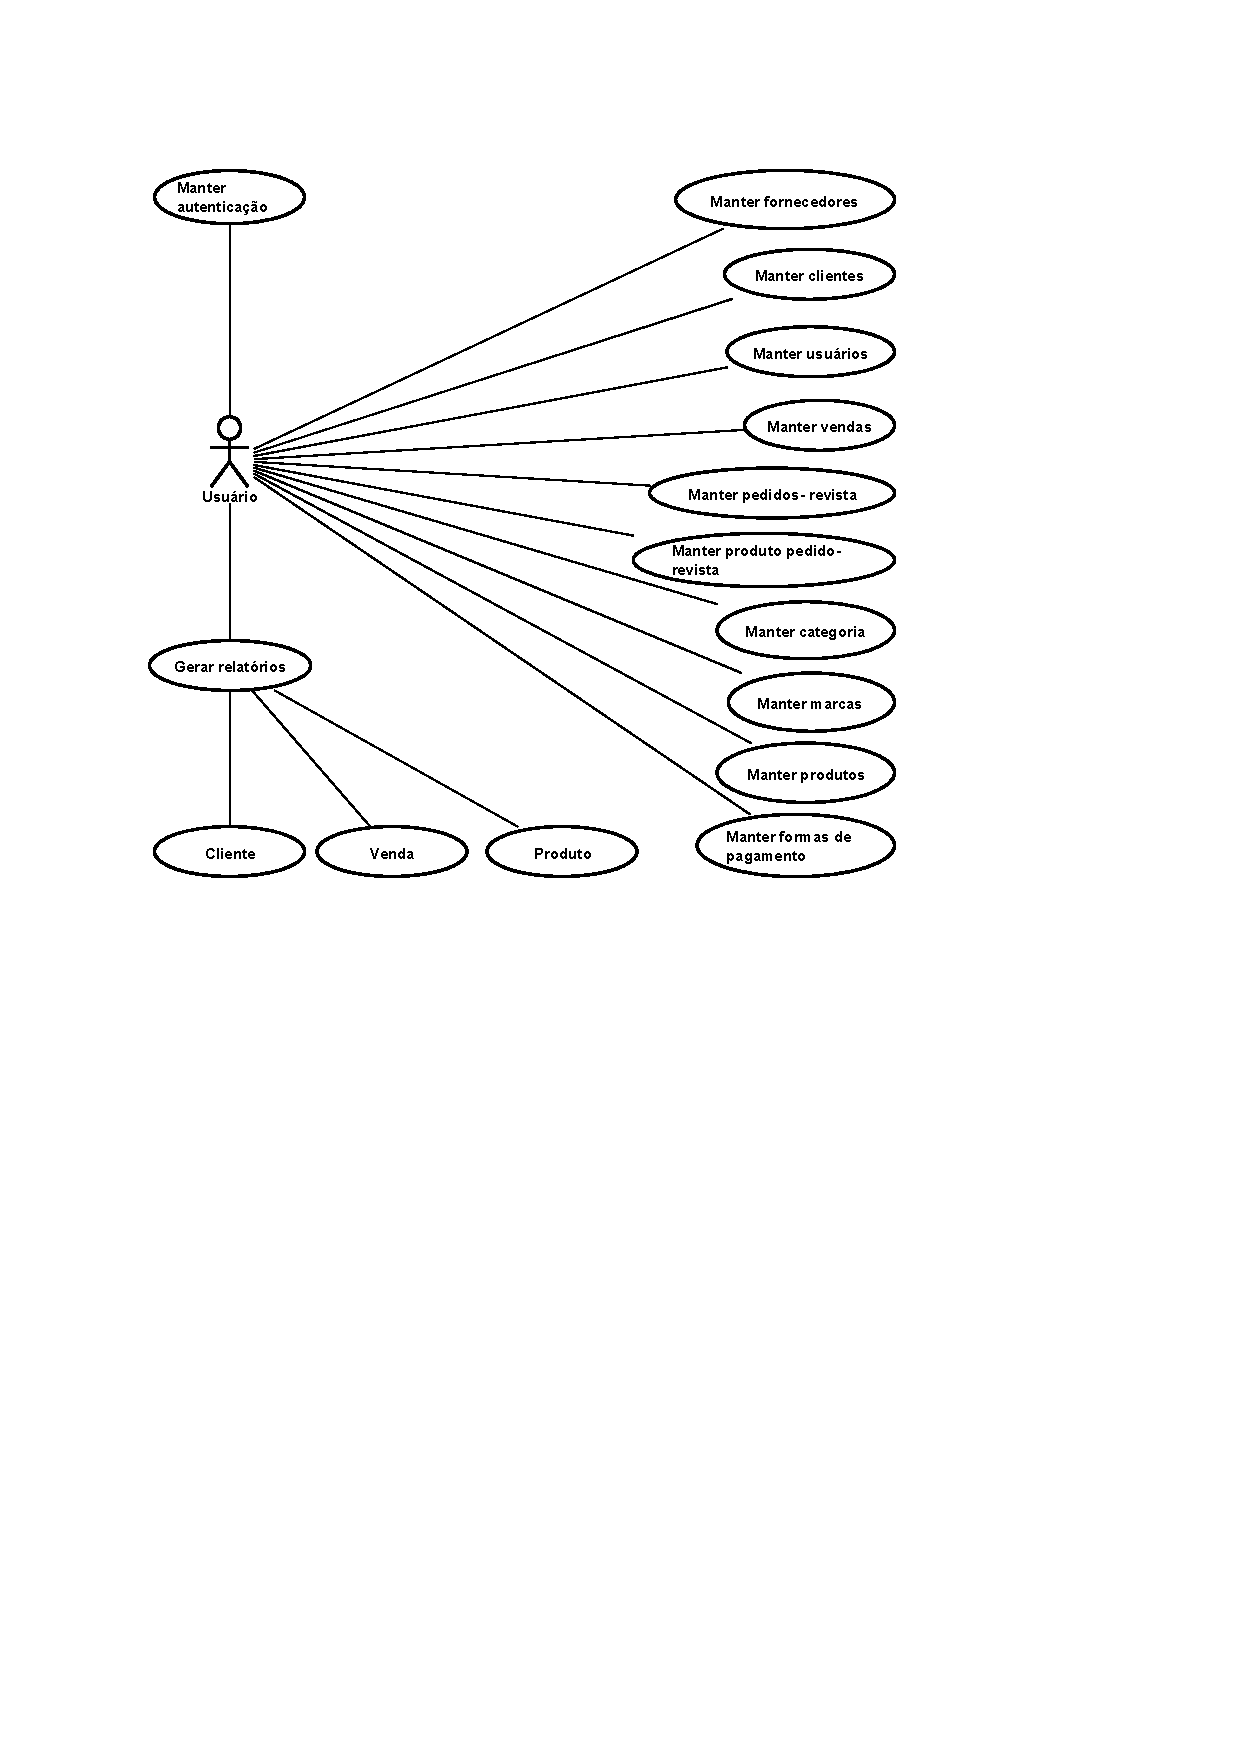
\includegraphics[scale=1.2]{uc.pdf}\caption{Diagrama de Caso de Uso}
\end{figure}

%=================================
\section{Diagrama de Classe}
\subsection{Atributos - Entidade}
\begin{figure}[H]\centering
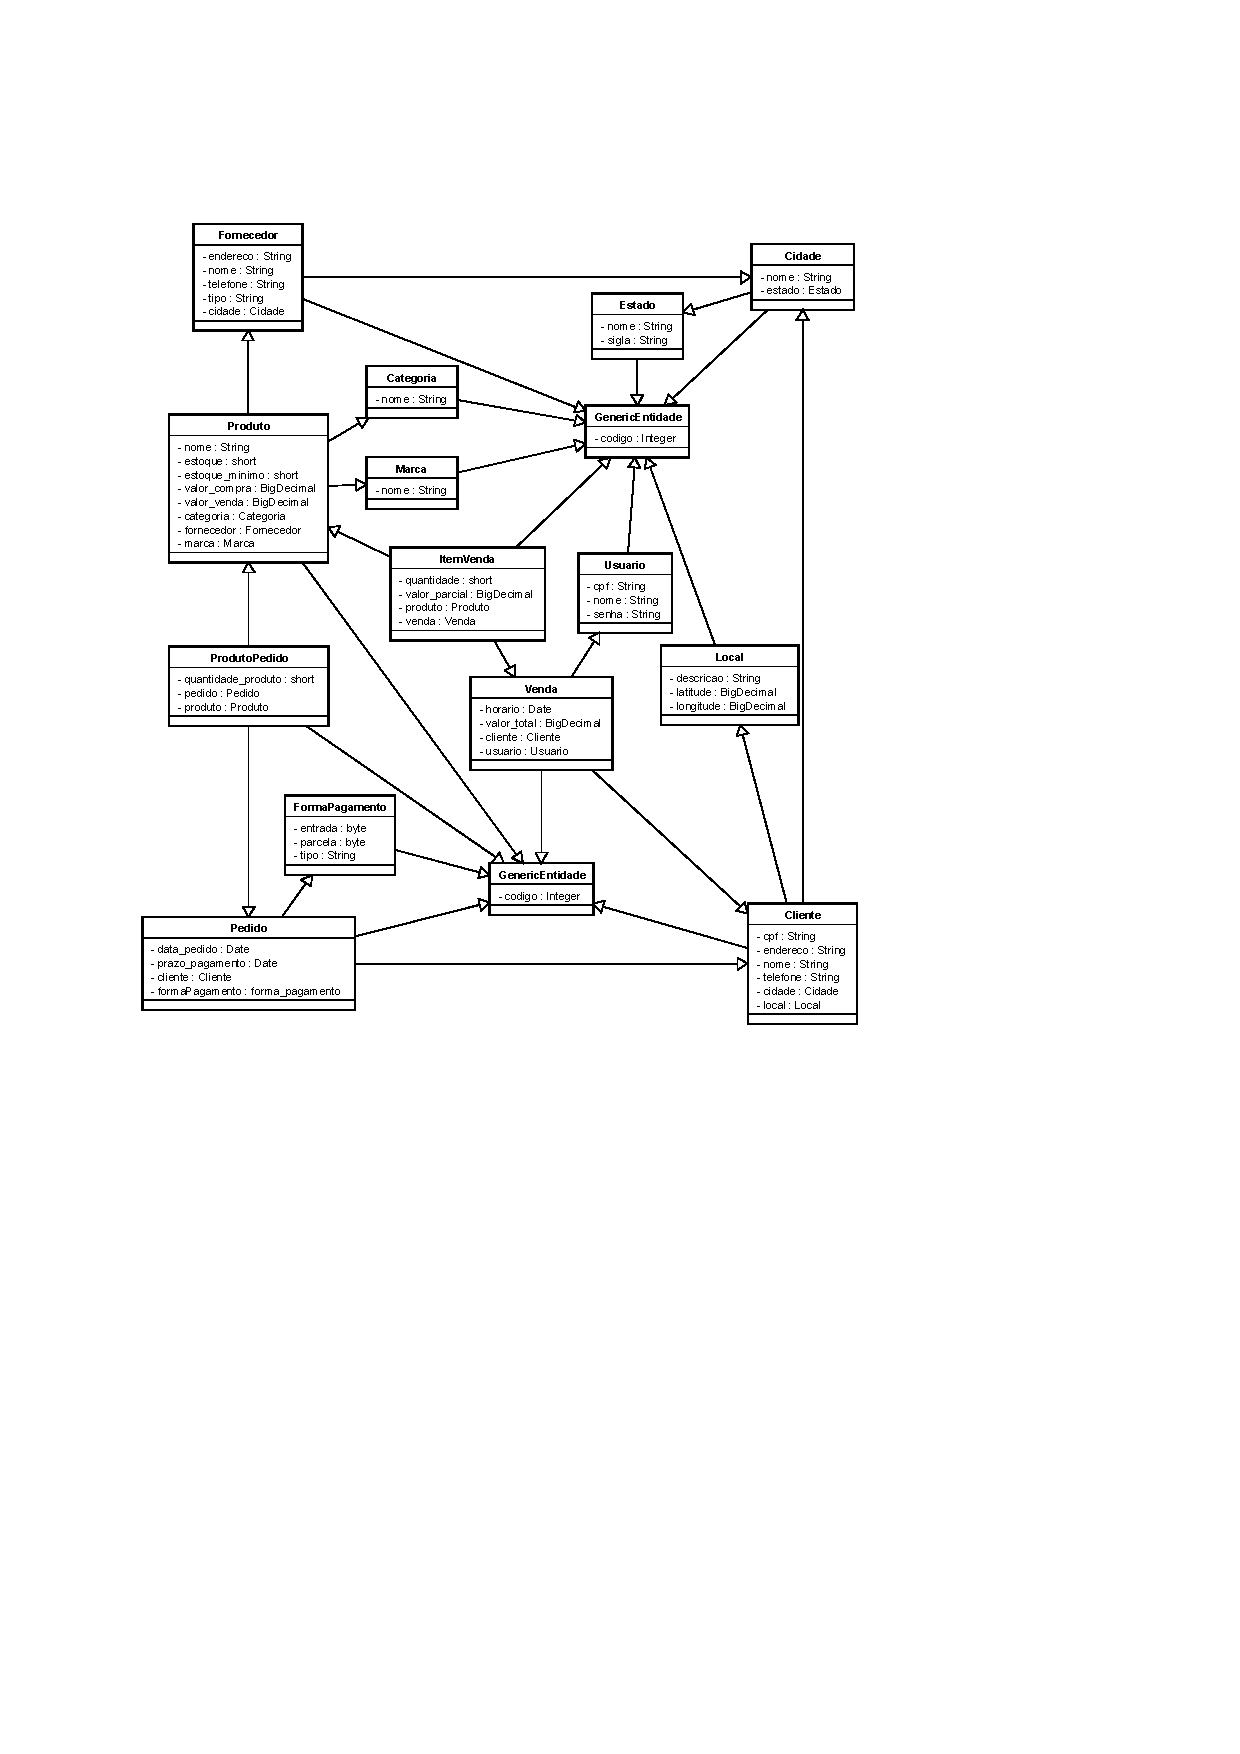
\includegraphics[scale=1.31]{atributo.pdf}\caption{Atributos}
\end{figure}

\newpage
\subsection{Métodos Dao}
\begin{figure}[h]\centering
	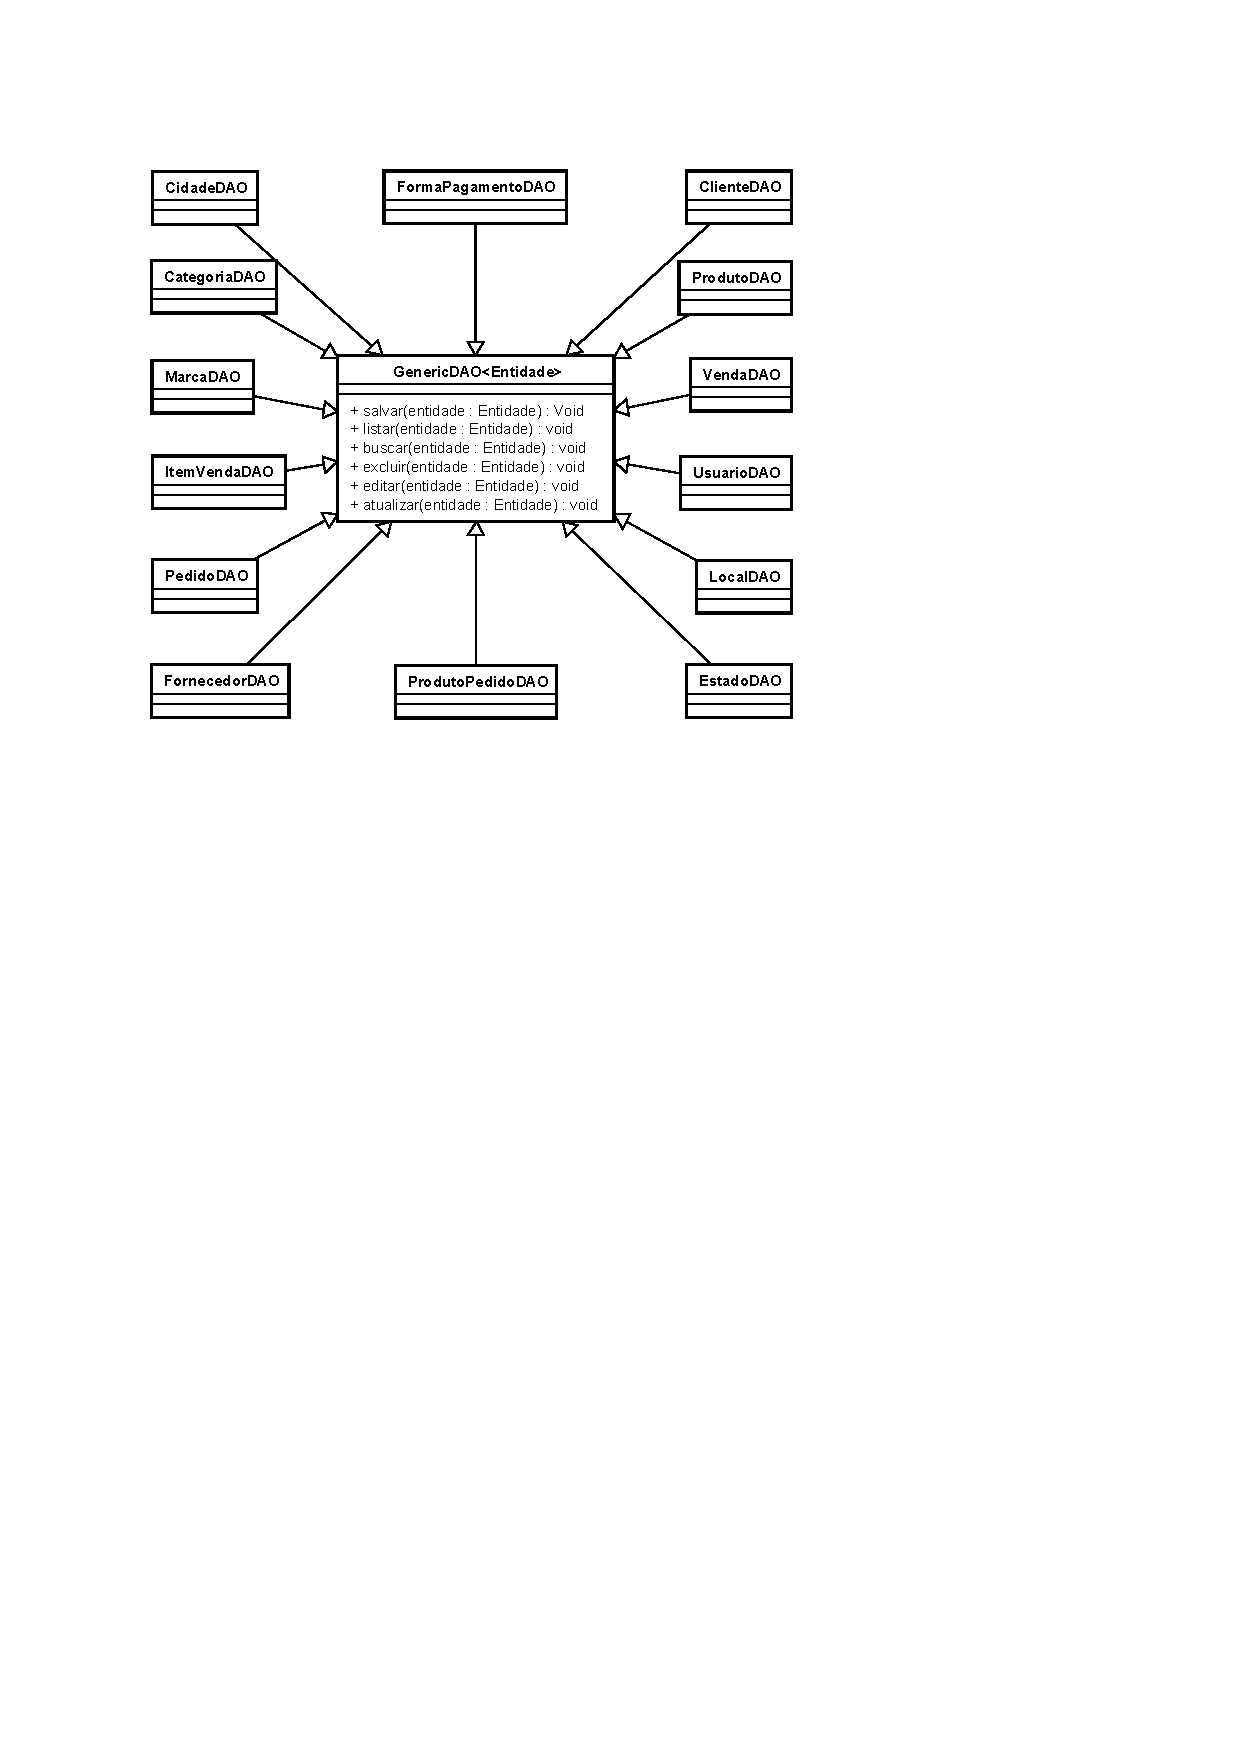
\includegraphics[scale=1.45]{metodo-dao.pdf}\caption{Métodos Dao}
\end{figure}

\newpage
\subsection{Métodos Bean}
\begin{figure}[h]\centering
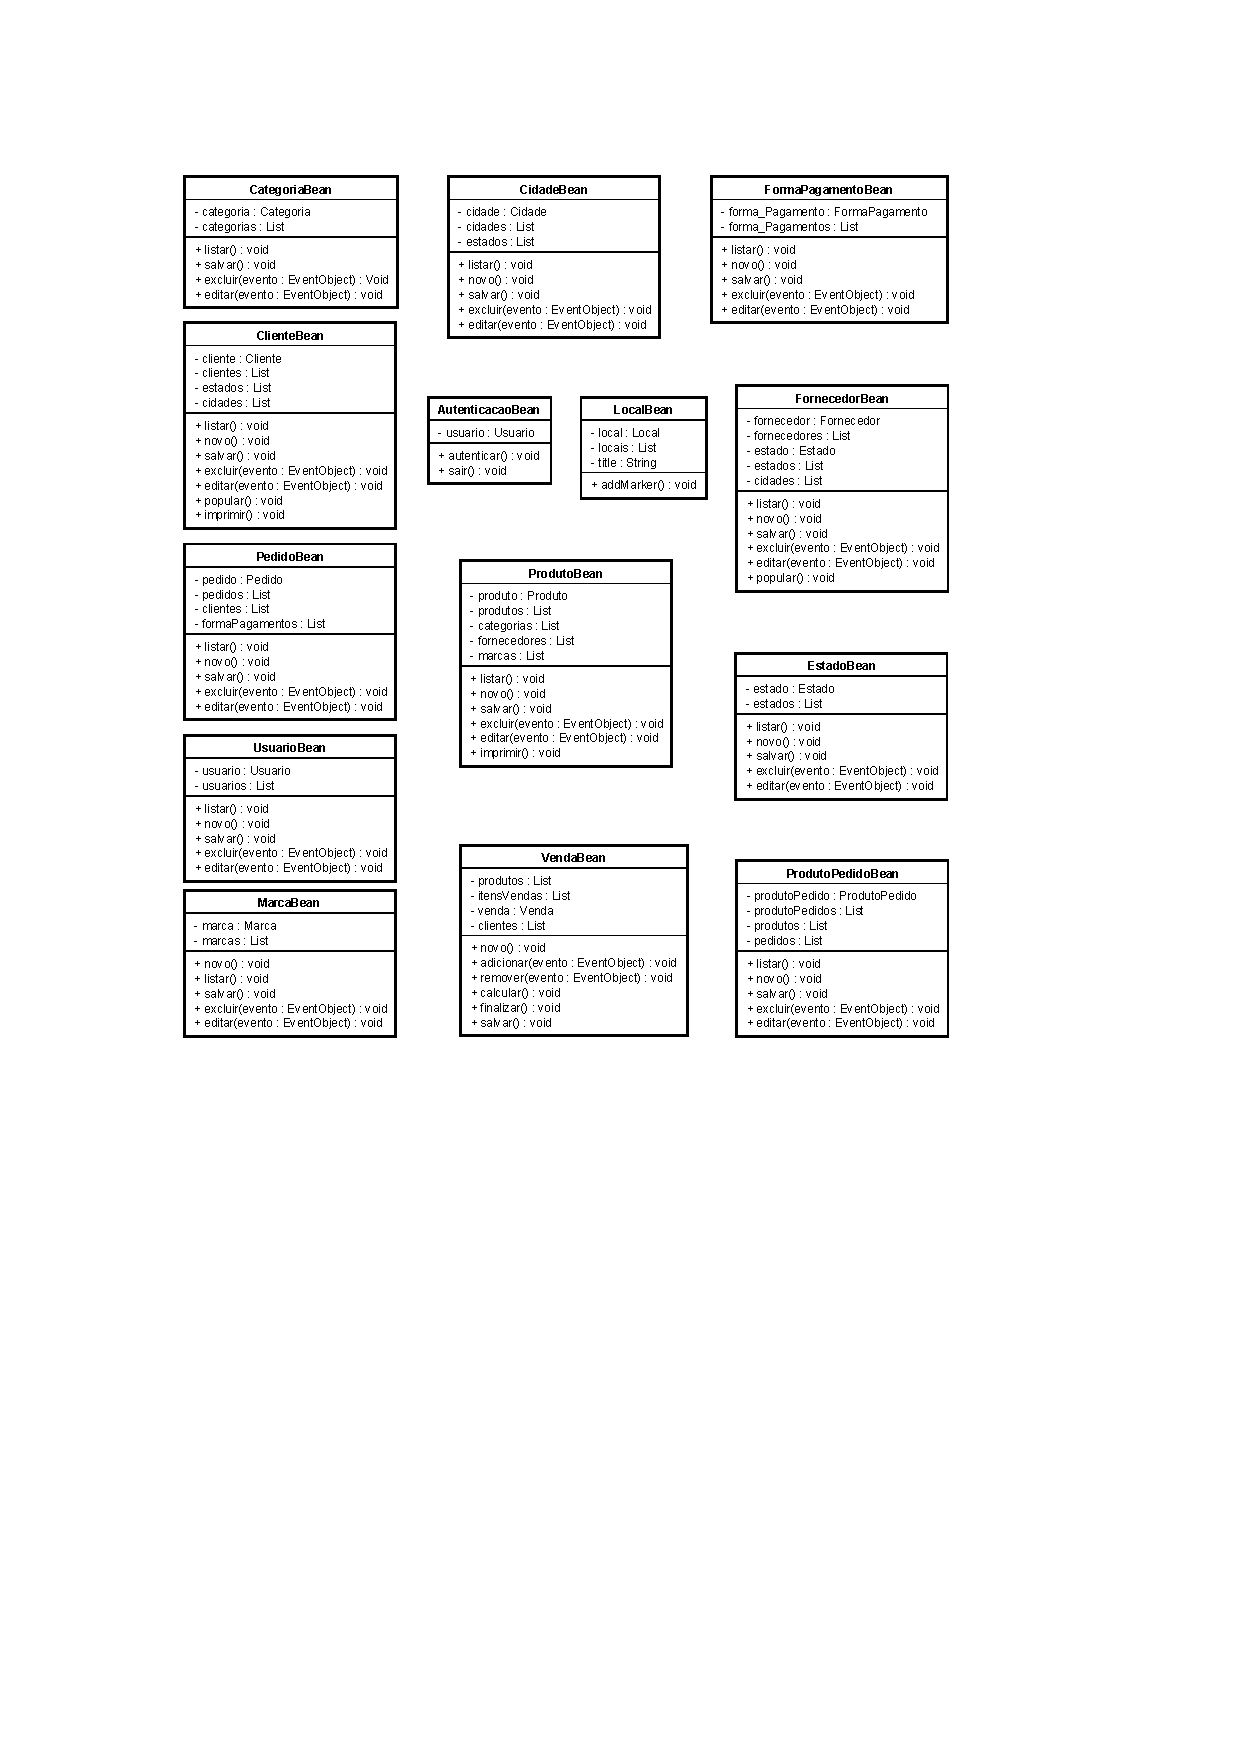
\includegraphics[scale=1.2]{metodo-bean.pdf}\caption{Métodos Bean}
\end{figure}

\newpage
\section{Diagrama de Atividade}
\subsection{Manter Autenticação}
\begin{figure}[h]\centering
	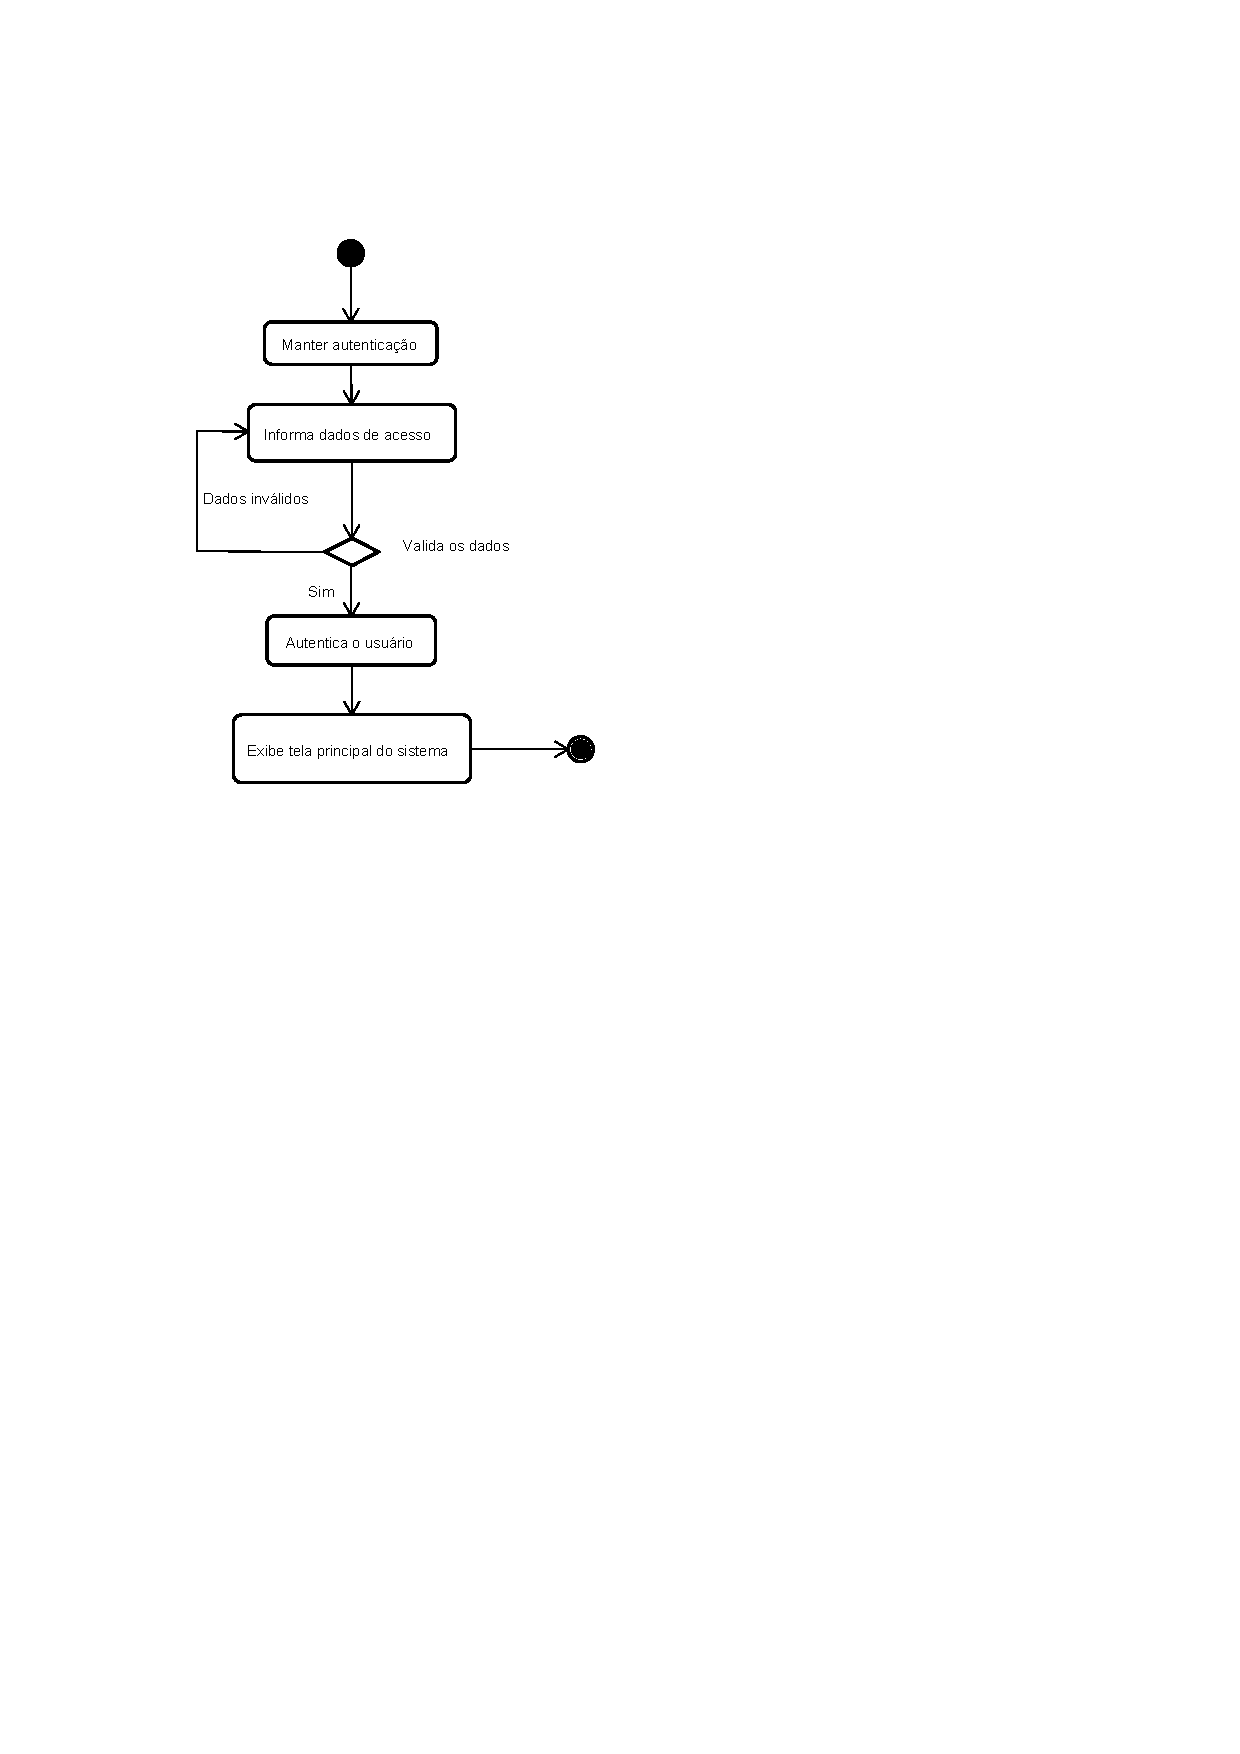
\includegraphics[scale=1.6]{autenticacao.pdf}\caption{Manter autenticação}
\end{figure}

\newpage
\subsection{Manter Fornecedor de Venda Tradicional e Direta}
\begin{figure}[h]\centering
	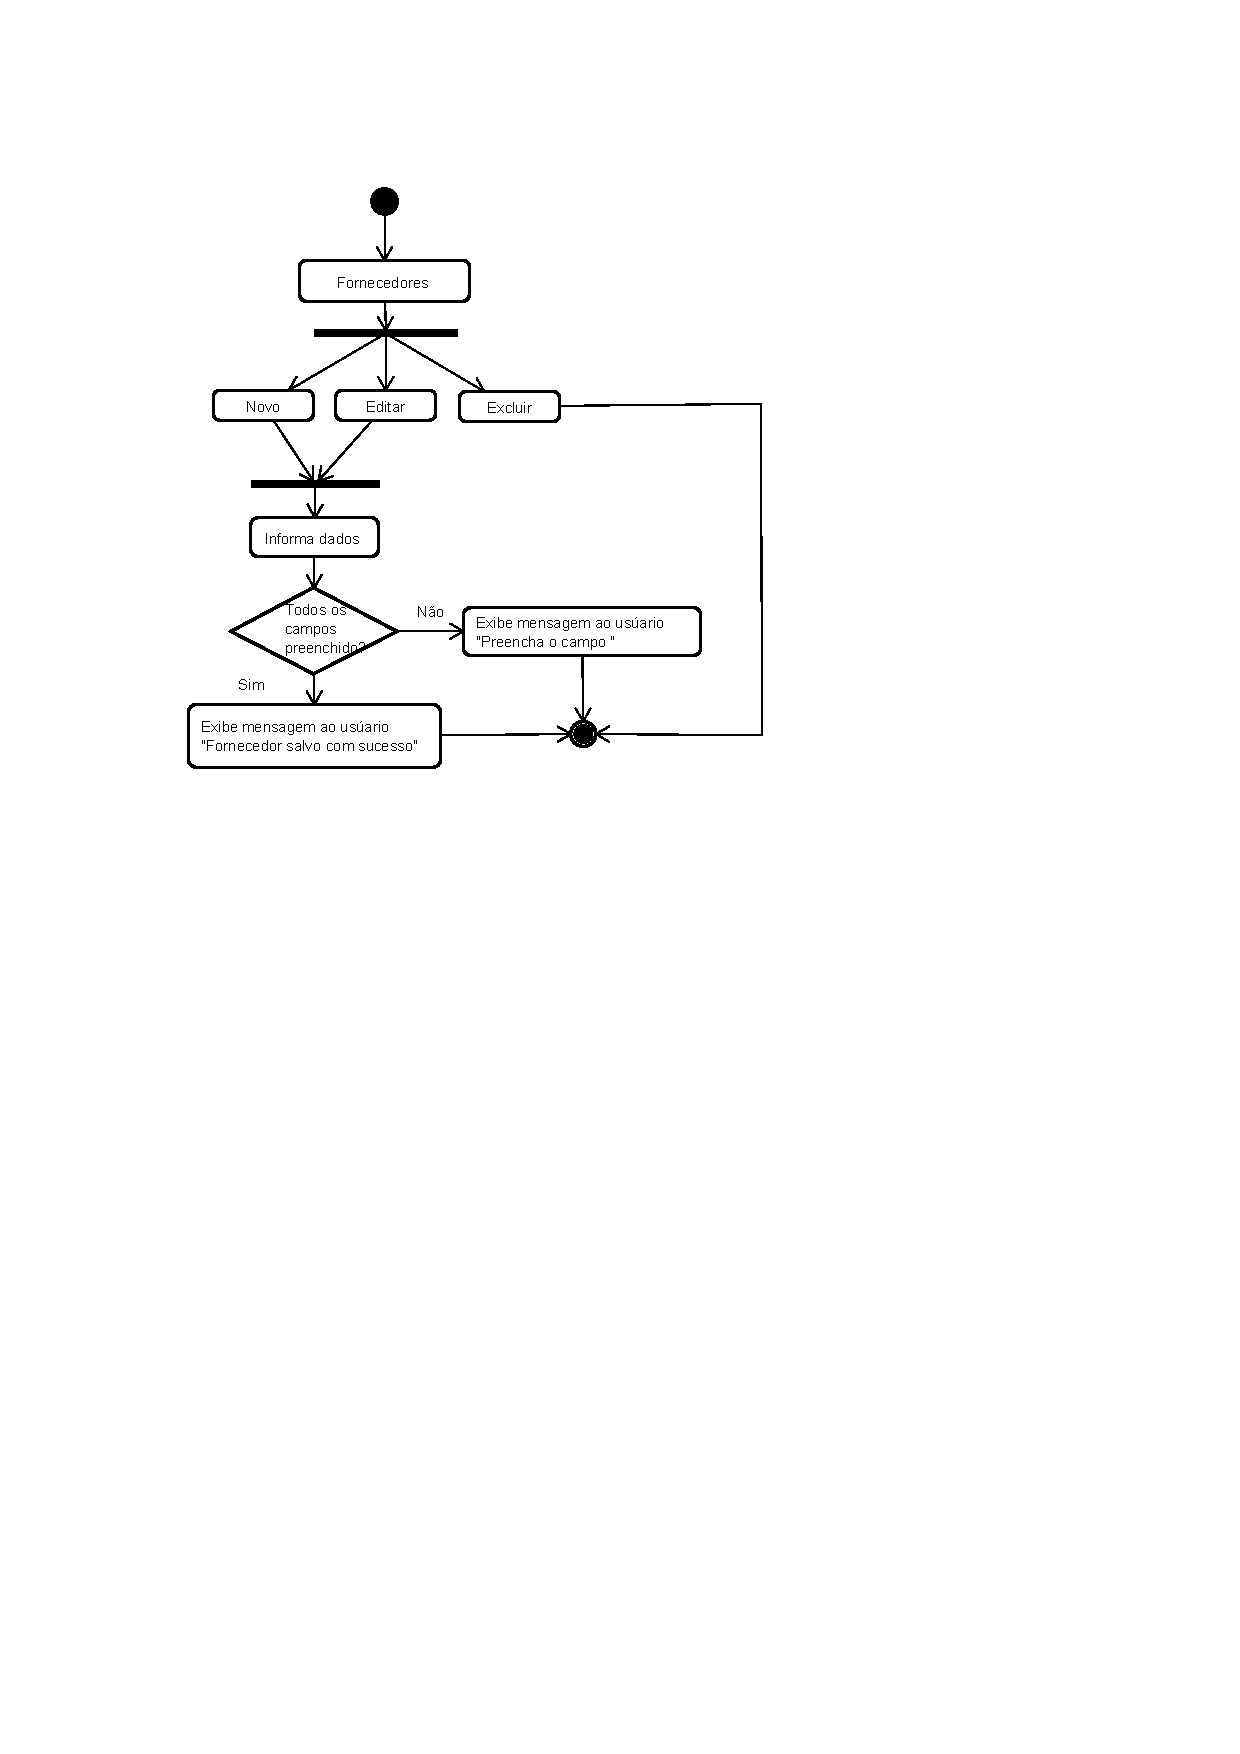
\includegraphics[scale=1.6]{fornecedor.pdf}\caption{Manter fornecedor de venda tradicional e direta}
\end{figure}

\newpage
\subsection{Manter Produto}
\begin{figure}[h]\centering
	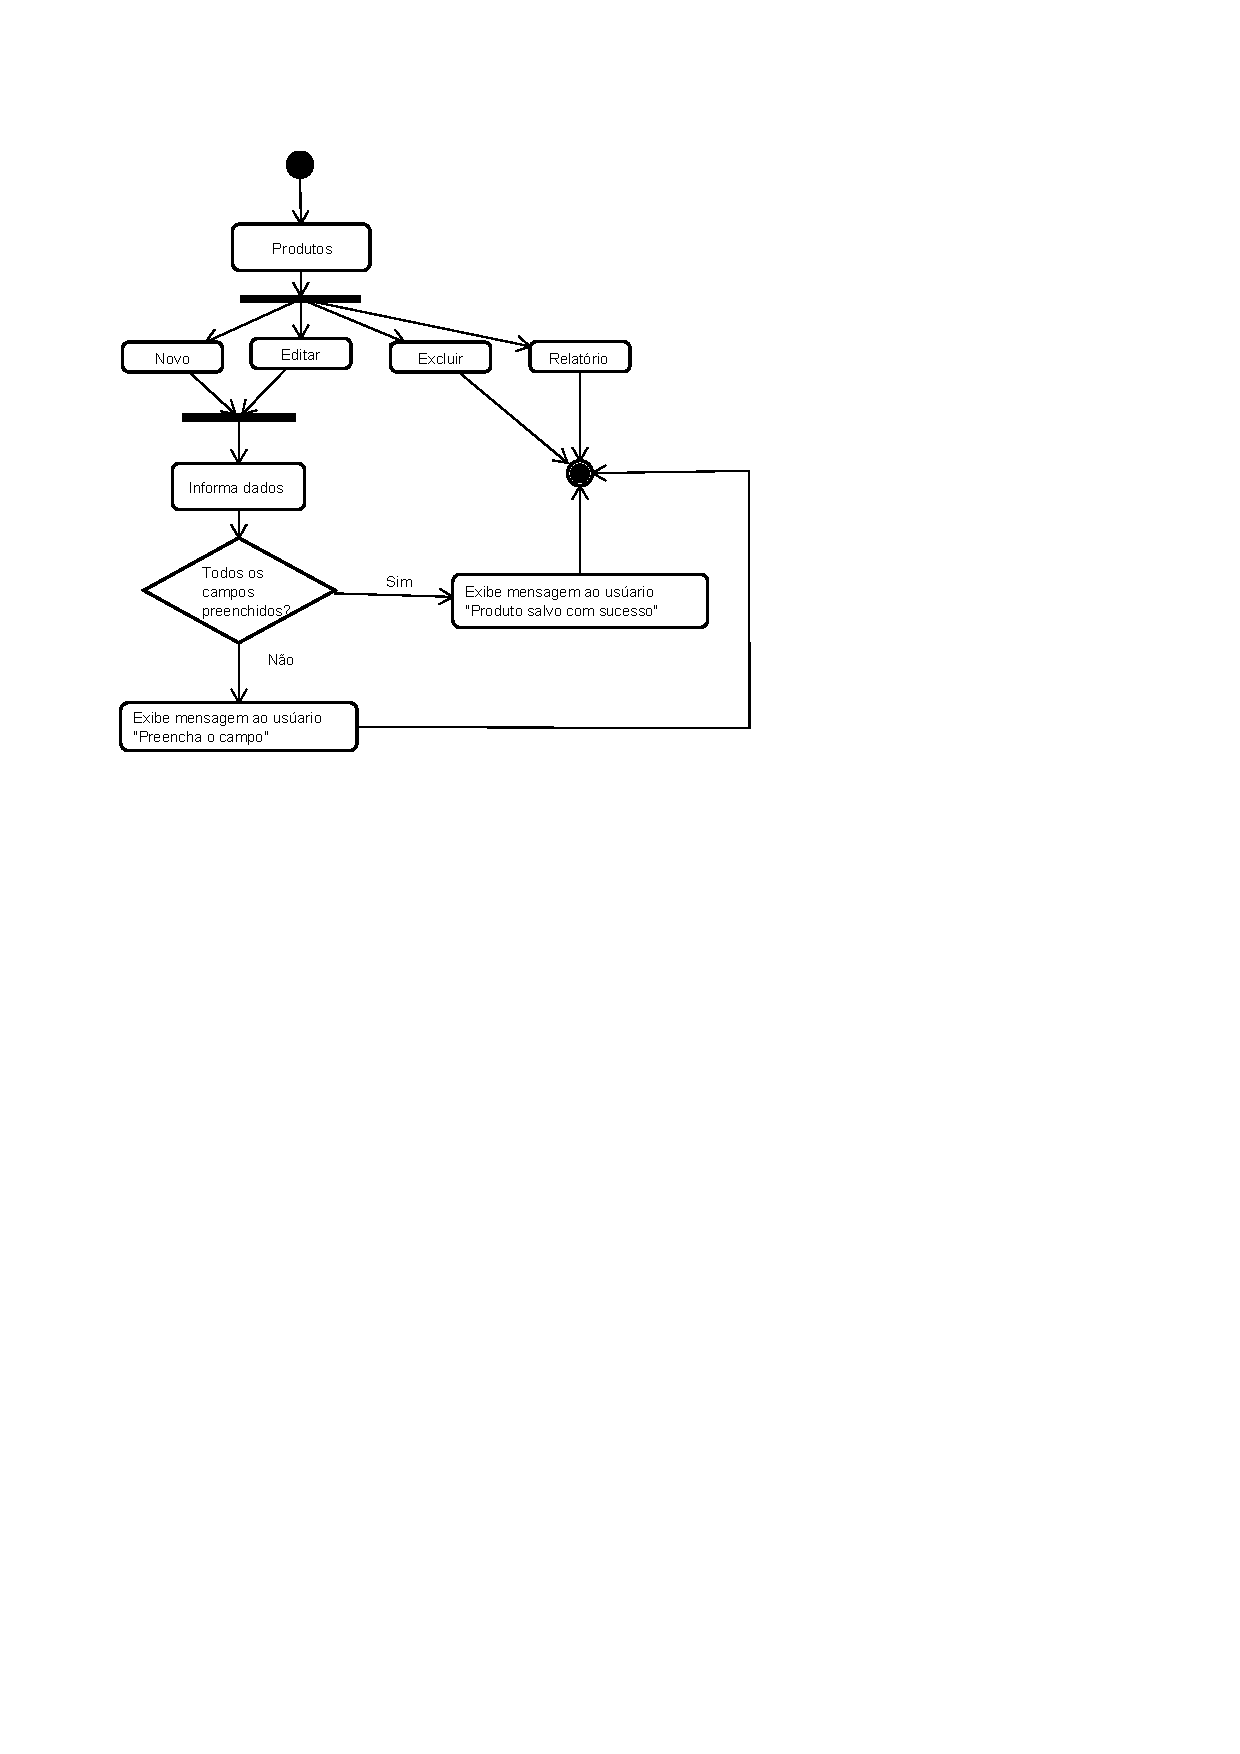
\includegraphics[scale=1.48]{produto.pdf}\caption{Manter produto}
\end{figure}

\newpage
\subsection{Manter Pedido - Revista}
\begin{figure}[h]\centering
	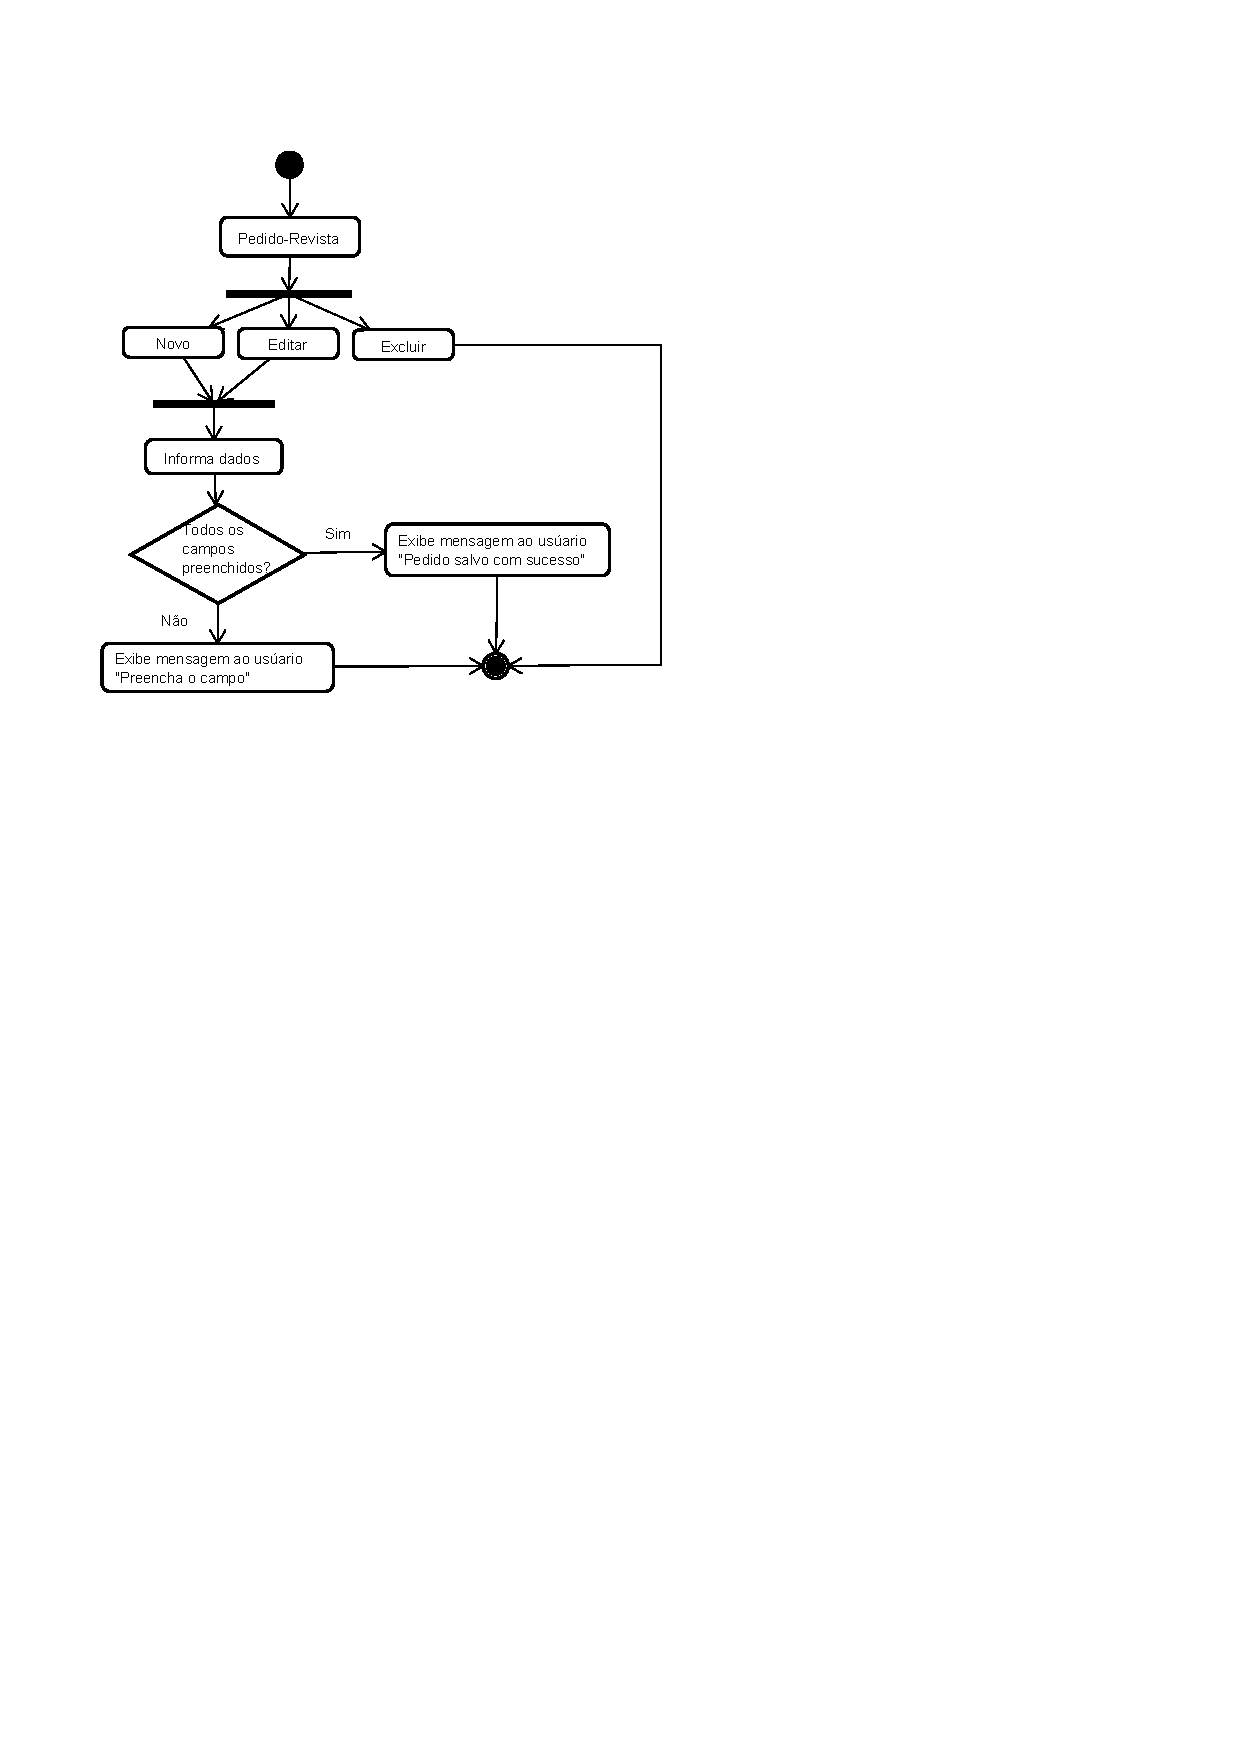
\includegraphics[scale=1.67]{pedido-revista.pdf}\caption{Manter pedido - revista}
\end{figure}

\newpage
\subsection{Manter Produto Pedido - Revista}
\begin{figure}[h]\centering
	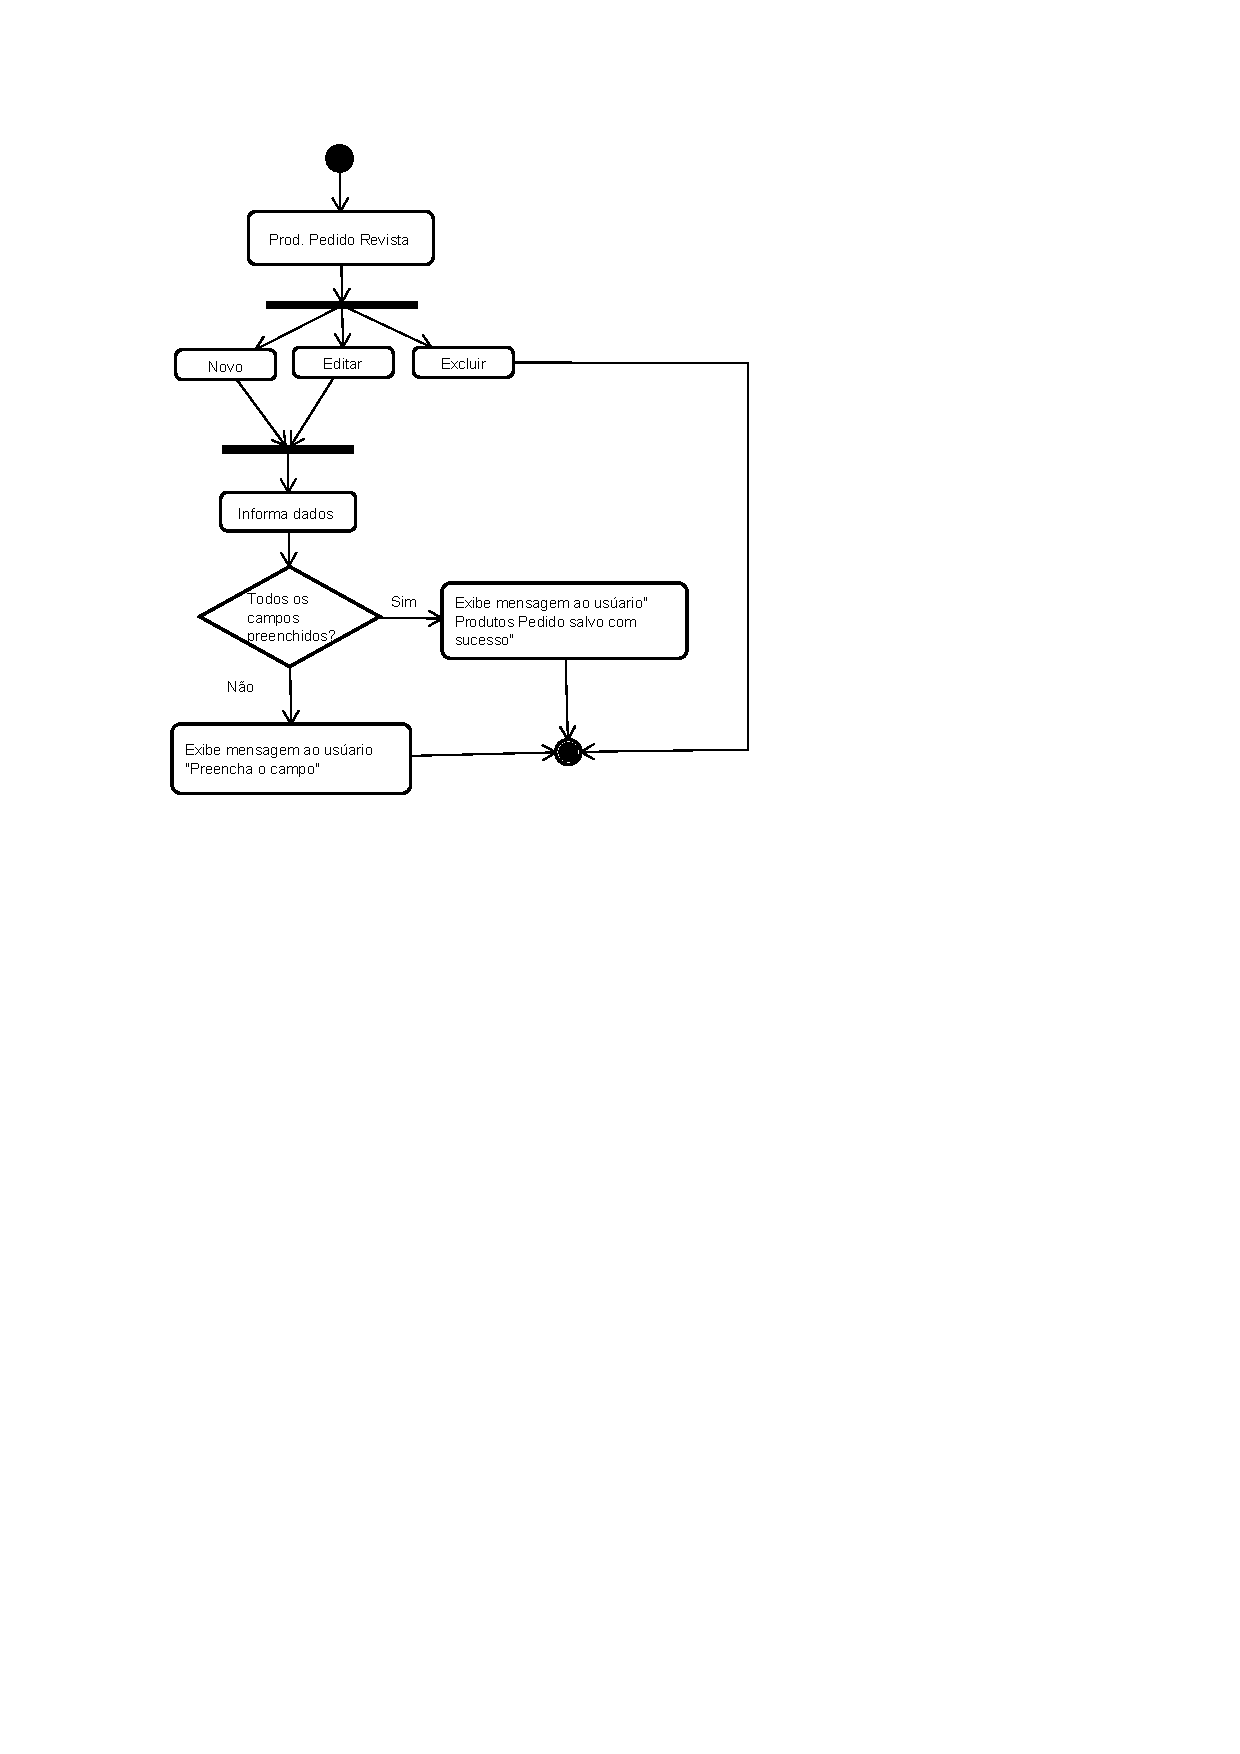
\includegraphics[scale=1.61]{produto-pedido-revista.pdf}\caption{Manter produto pedido - revista}
\end{figure}

\newpage
\subsection{Manter Cliente}
\begin{figure}[h]\centering
	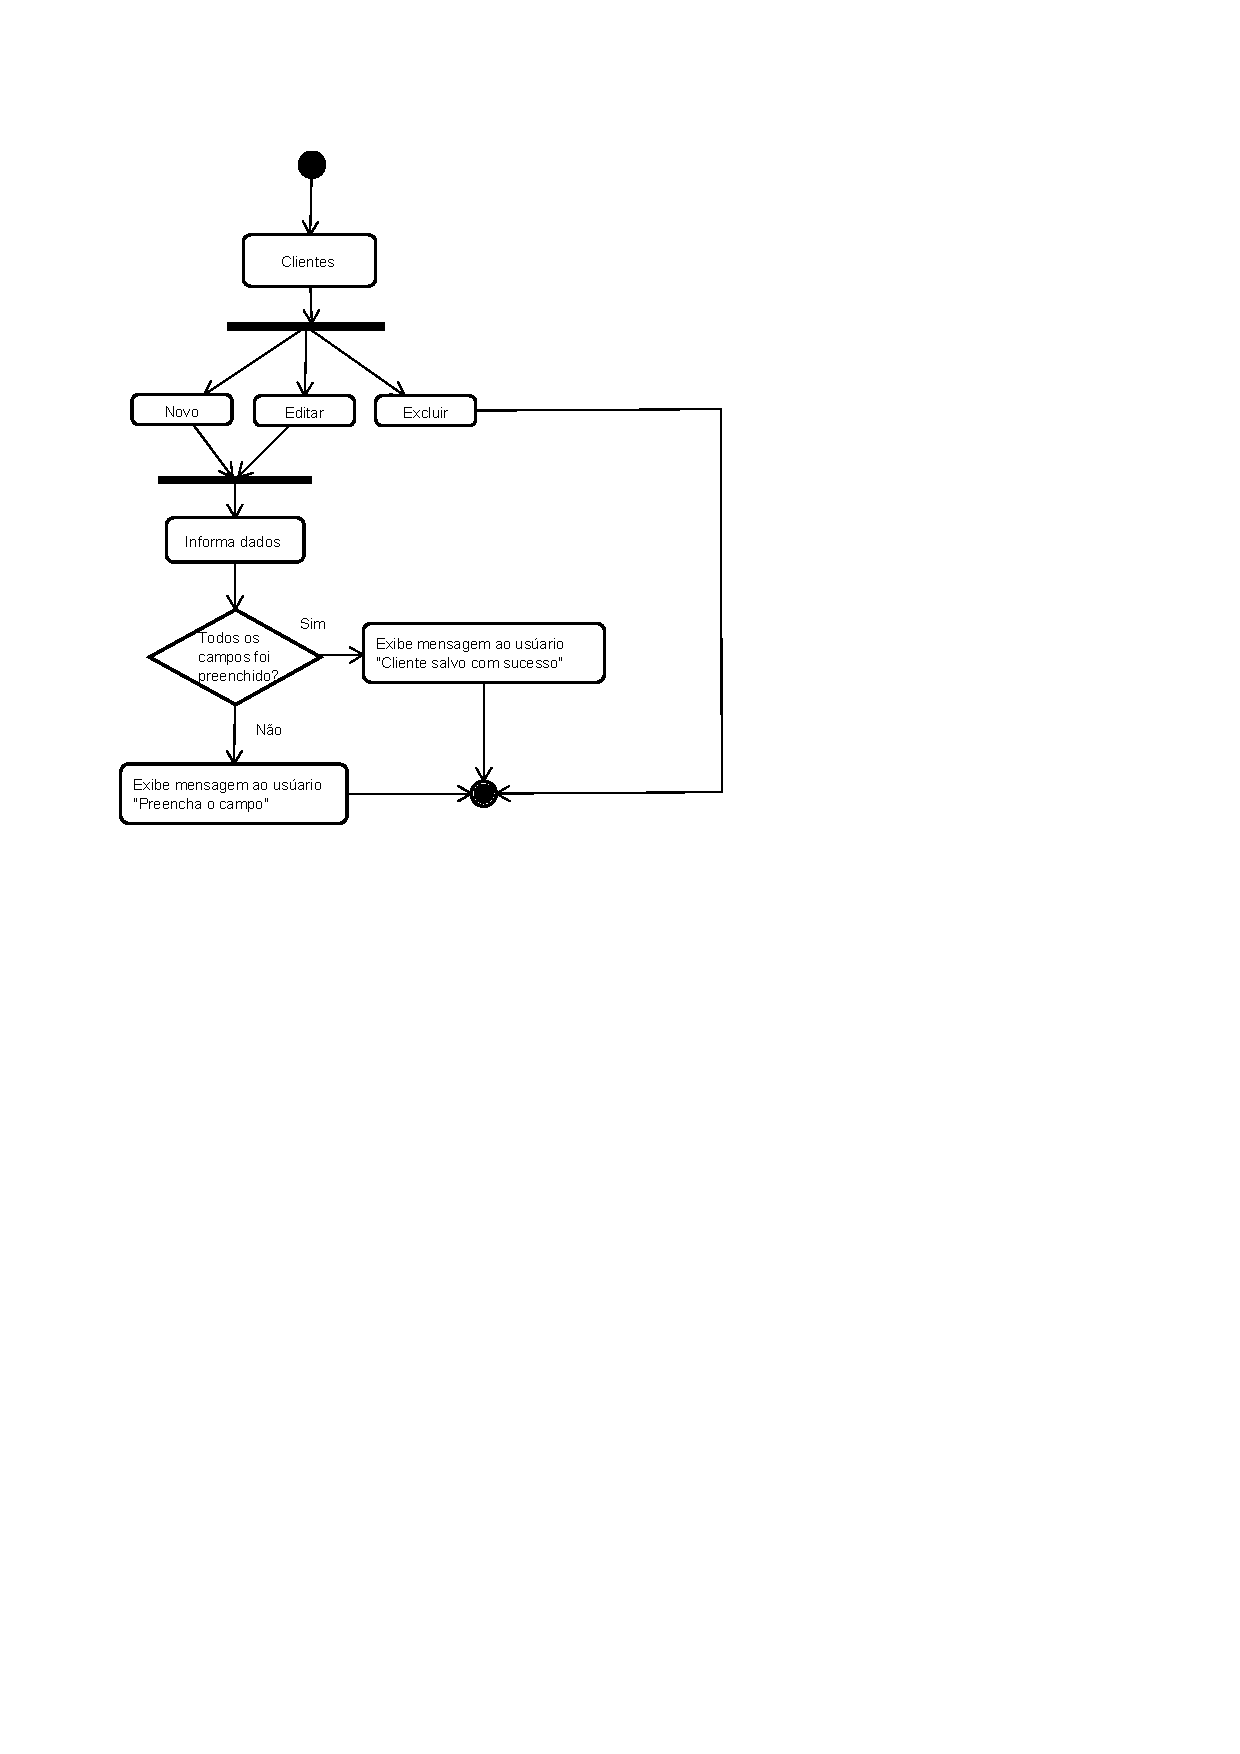
\includegraphics[scale=1.54]{cliente.pdf}\caption{Manter cliente}
\end{figure}

\newpage
\subsection{Emitir Relatório}
\begin{figure}[h]\centering
	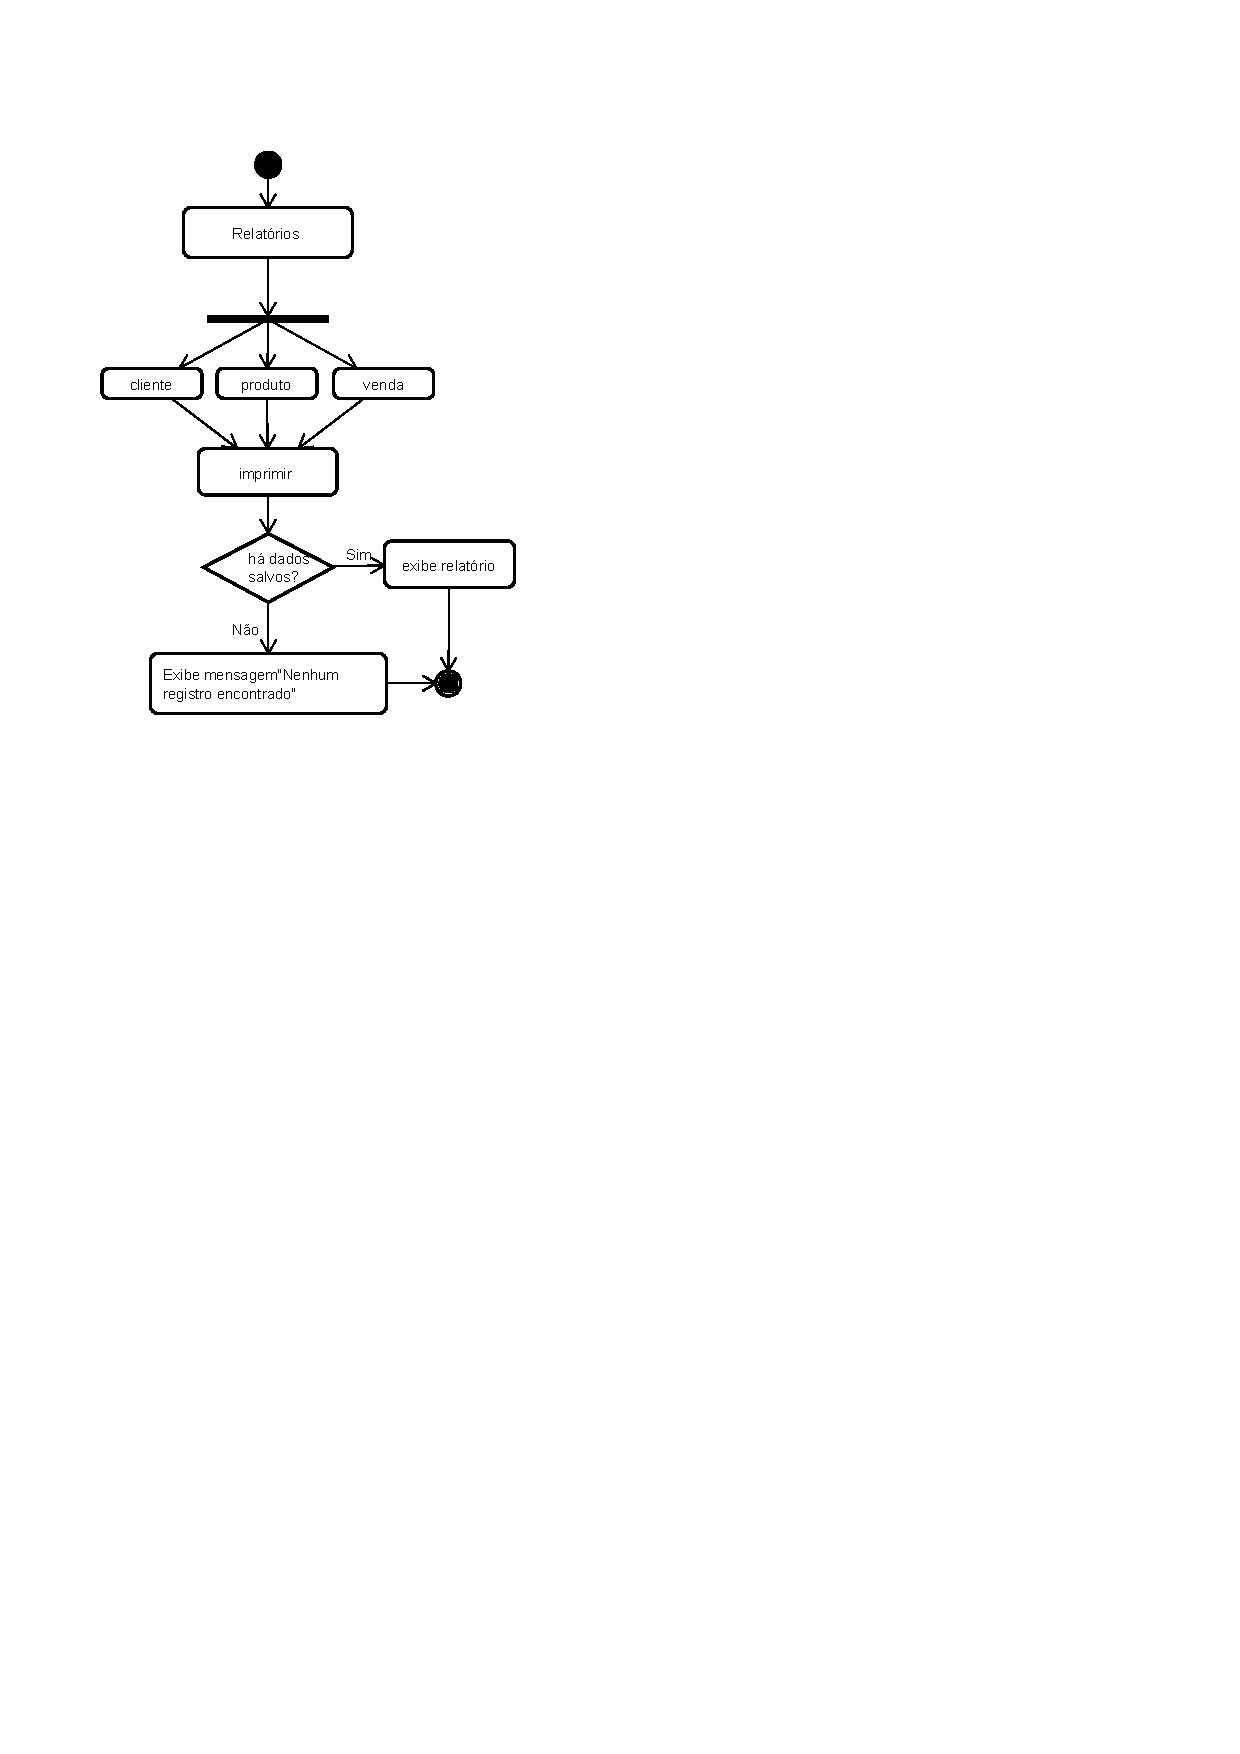
\includegraphics[scale=1.8]{emitir-relatorio.pdf}\caption{Emitir relatório}
\end{figure}

\newpage
\subsection{Manter Usuário}
\begin{figure}[h]\centering
	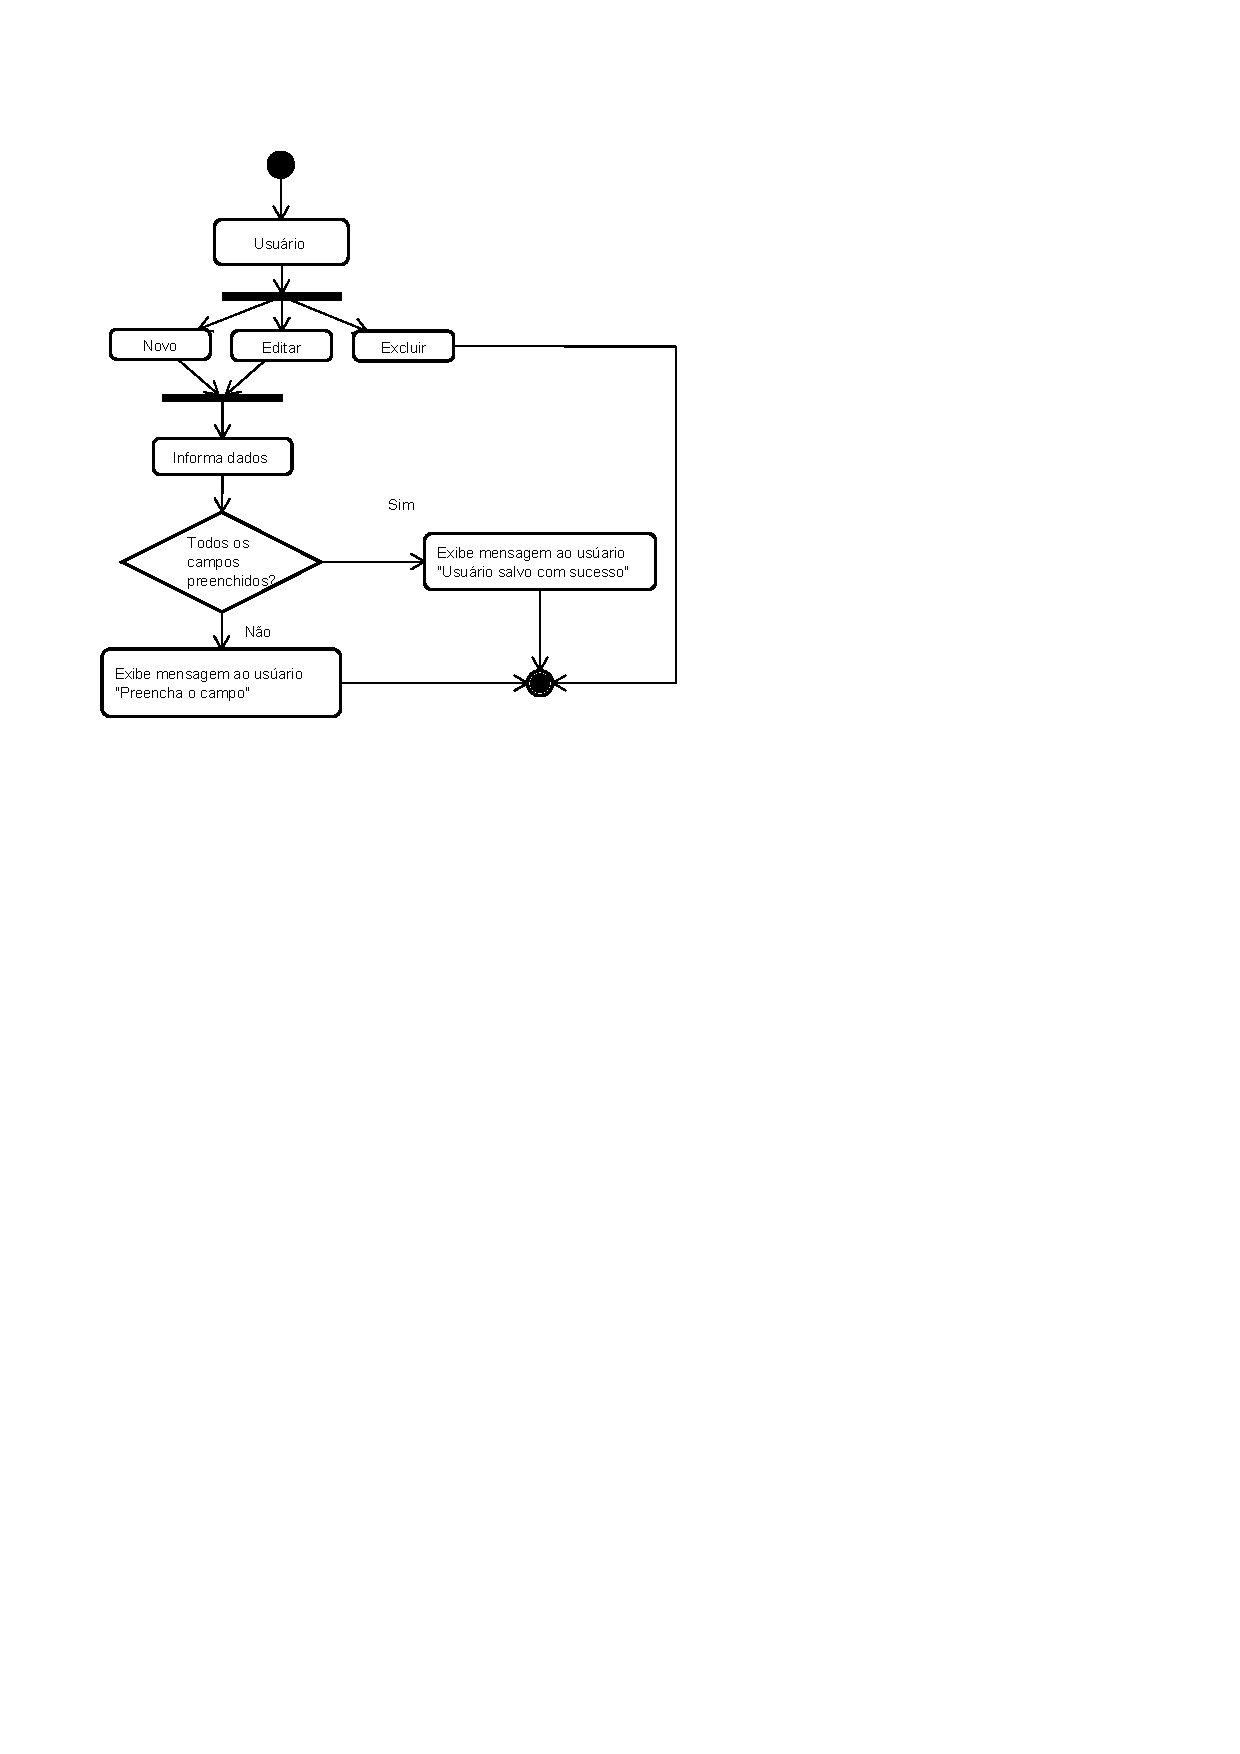
\includegraphics[scale=1.63]{usuario.pdf}\caption{Manter usuário}
\end{figure}

\newpage
\subsection{Manter Categoria}
\begin{figure}[h]\centering
	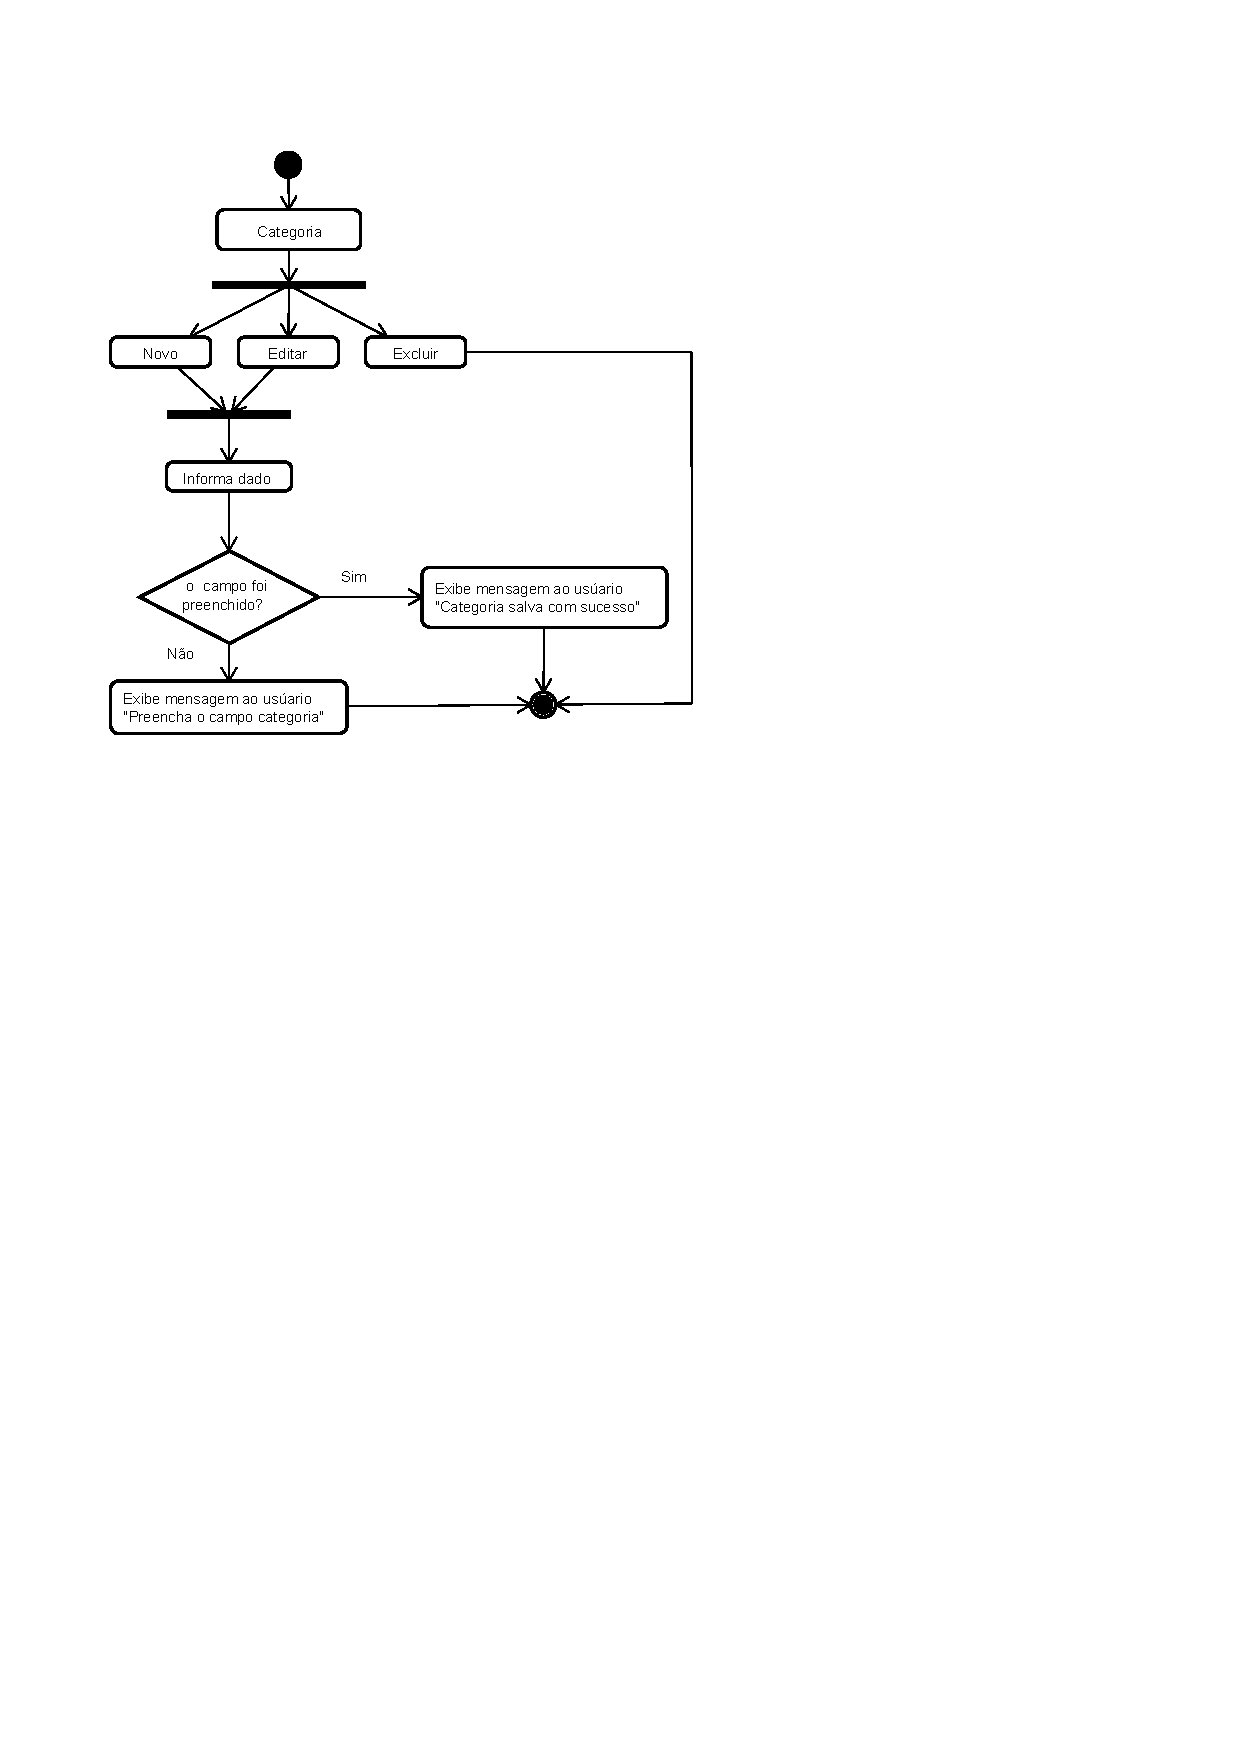
\includegraphics[scale=1.61]{categoria.pdf}\caption{Manter categoria}
\end{figure}

\newpage
\subsection{Manter Marca}
\begin{figure}[h]\centering
	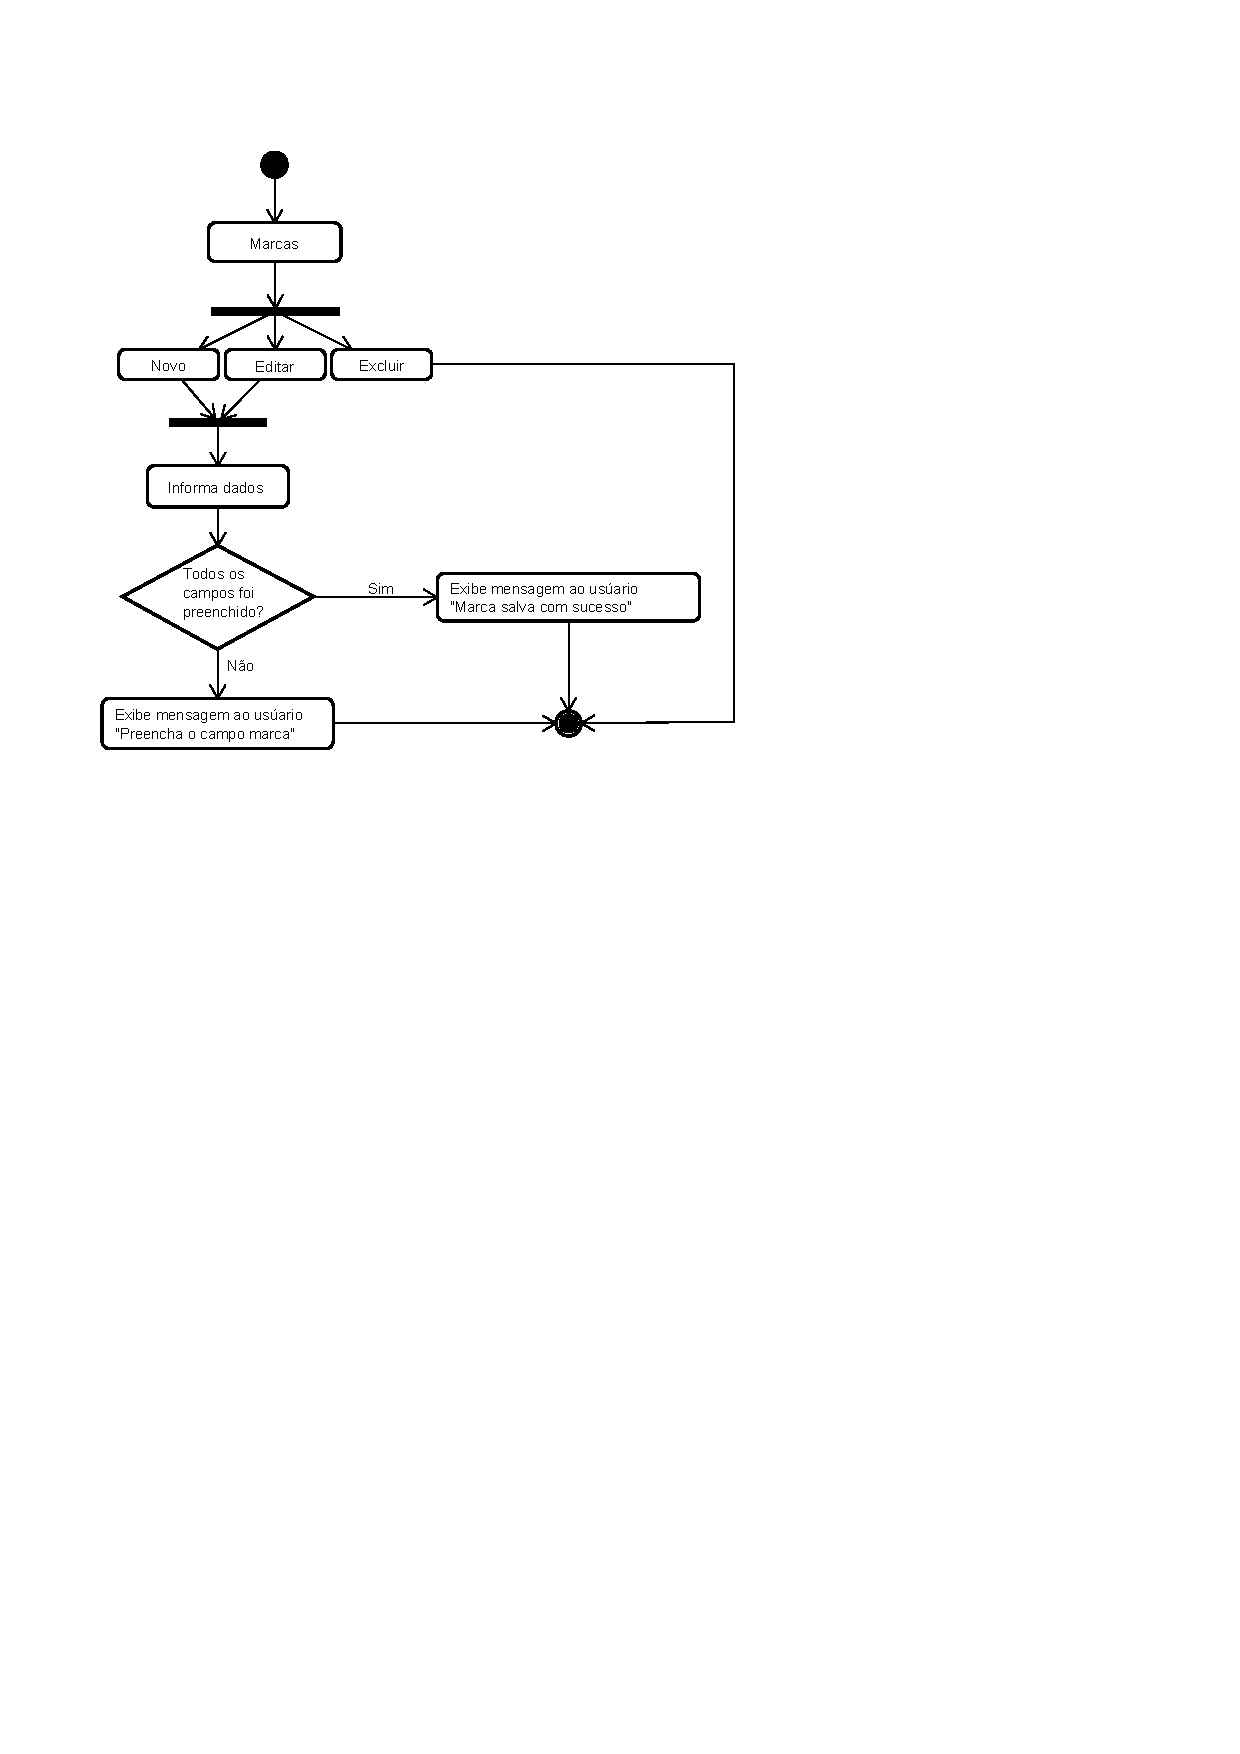
\includegraphics[scale=1.48]{marca.pdf}\caption{Manter marca}
\end{figure}

\newpage
\subsection{Manter Forma de Pagamento}
\begin{figure}[h]\centering
	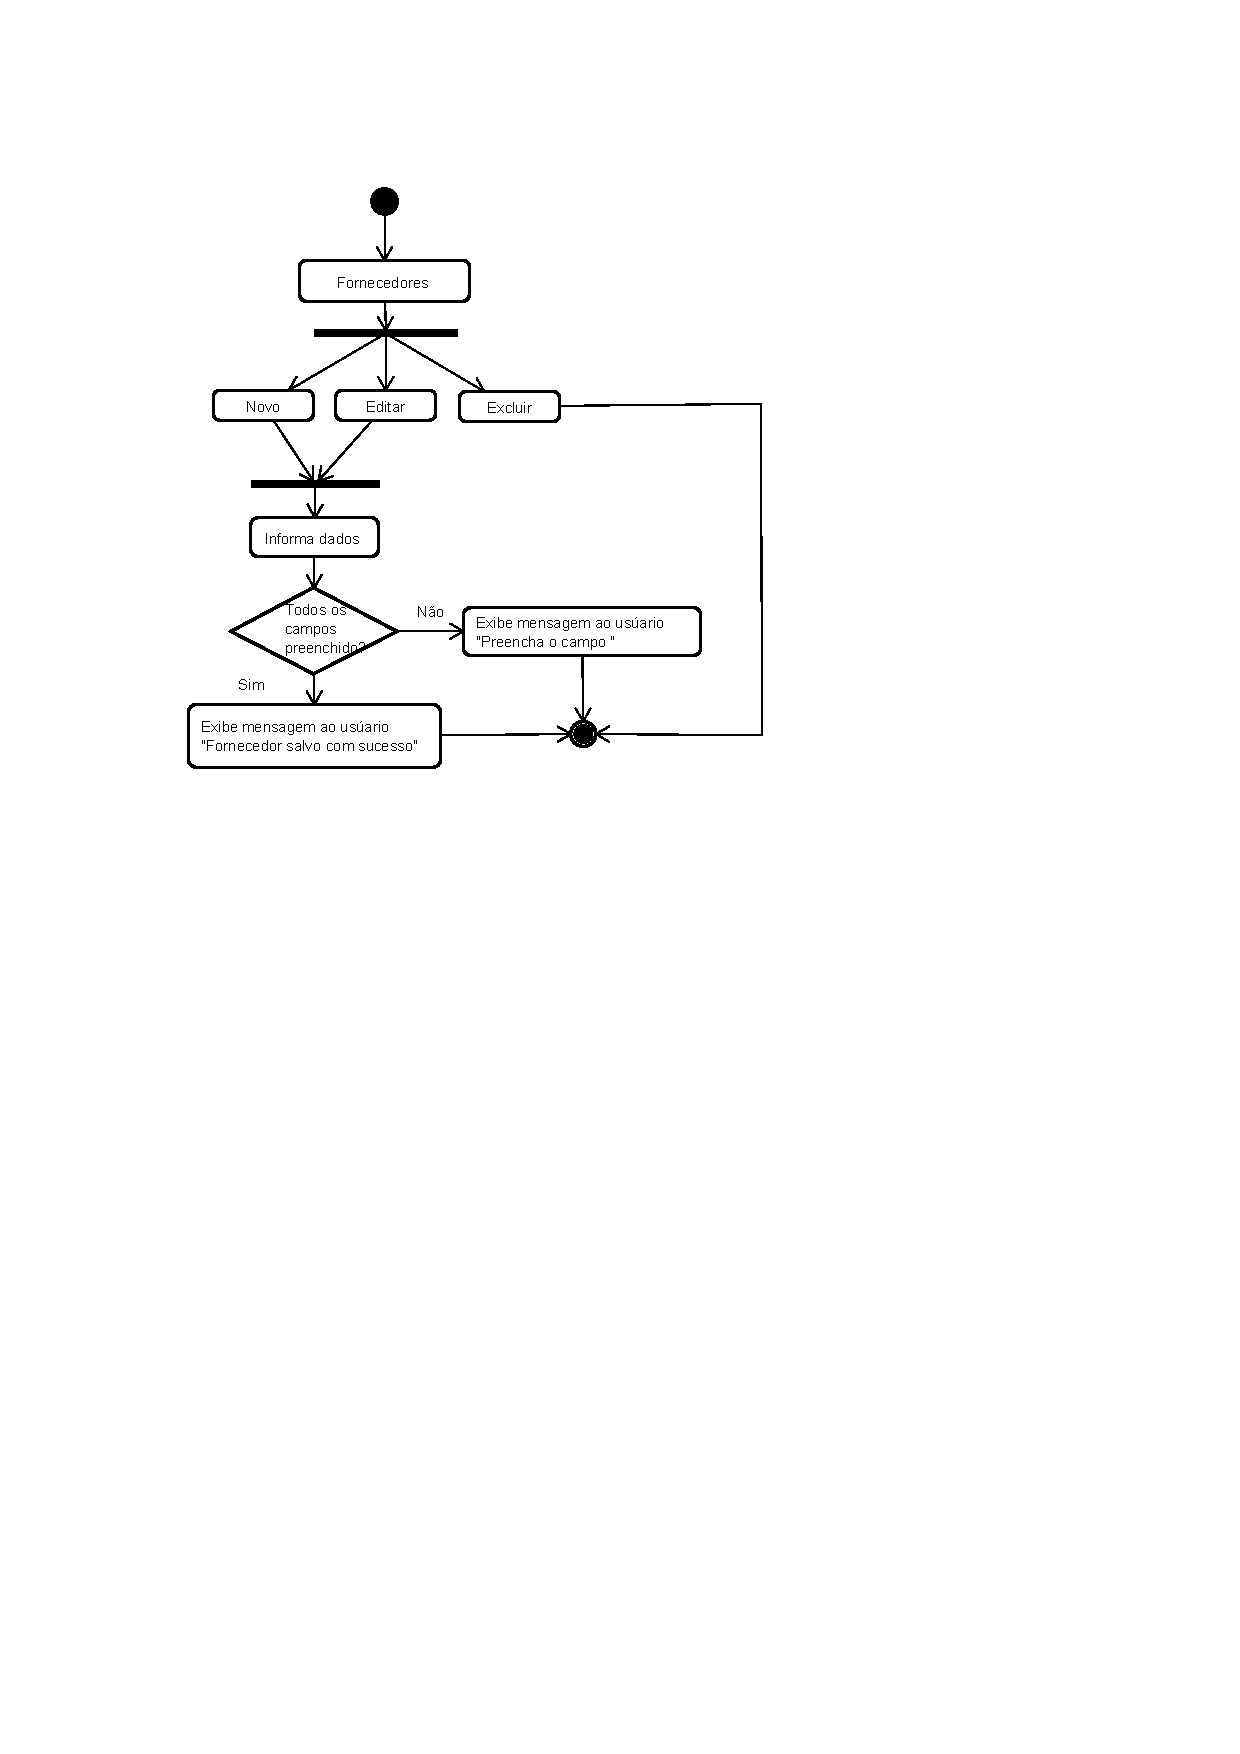
\includegraphics[scale=1.6]{fornecedor.pdf}\caption{Manter forma de pagamento}
\end{figure}

\newpage
\subsection{Manter Venda}
\begin{figure}[h]\centering
	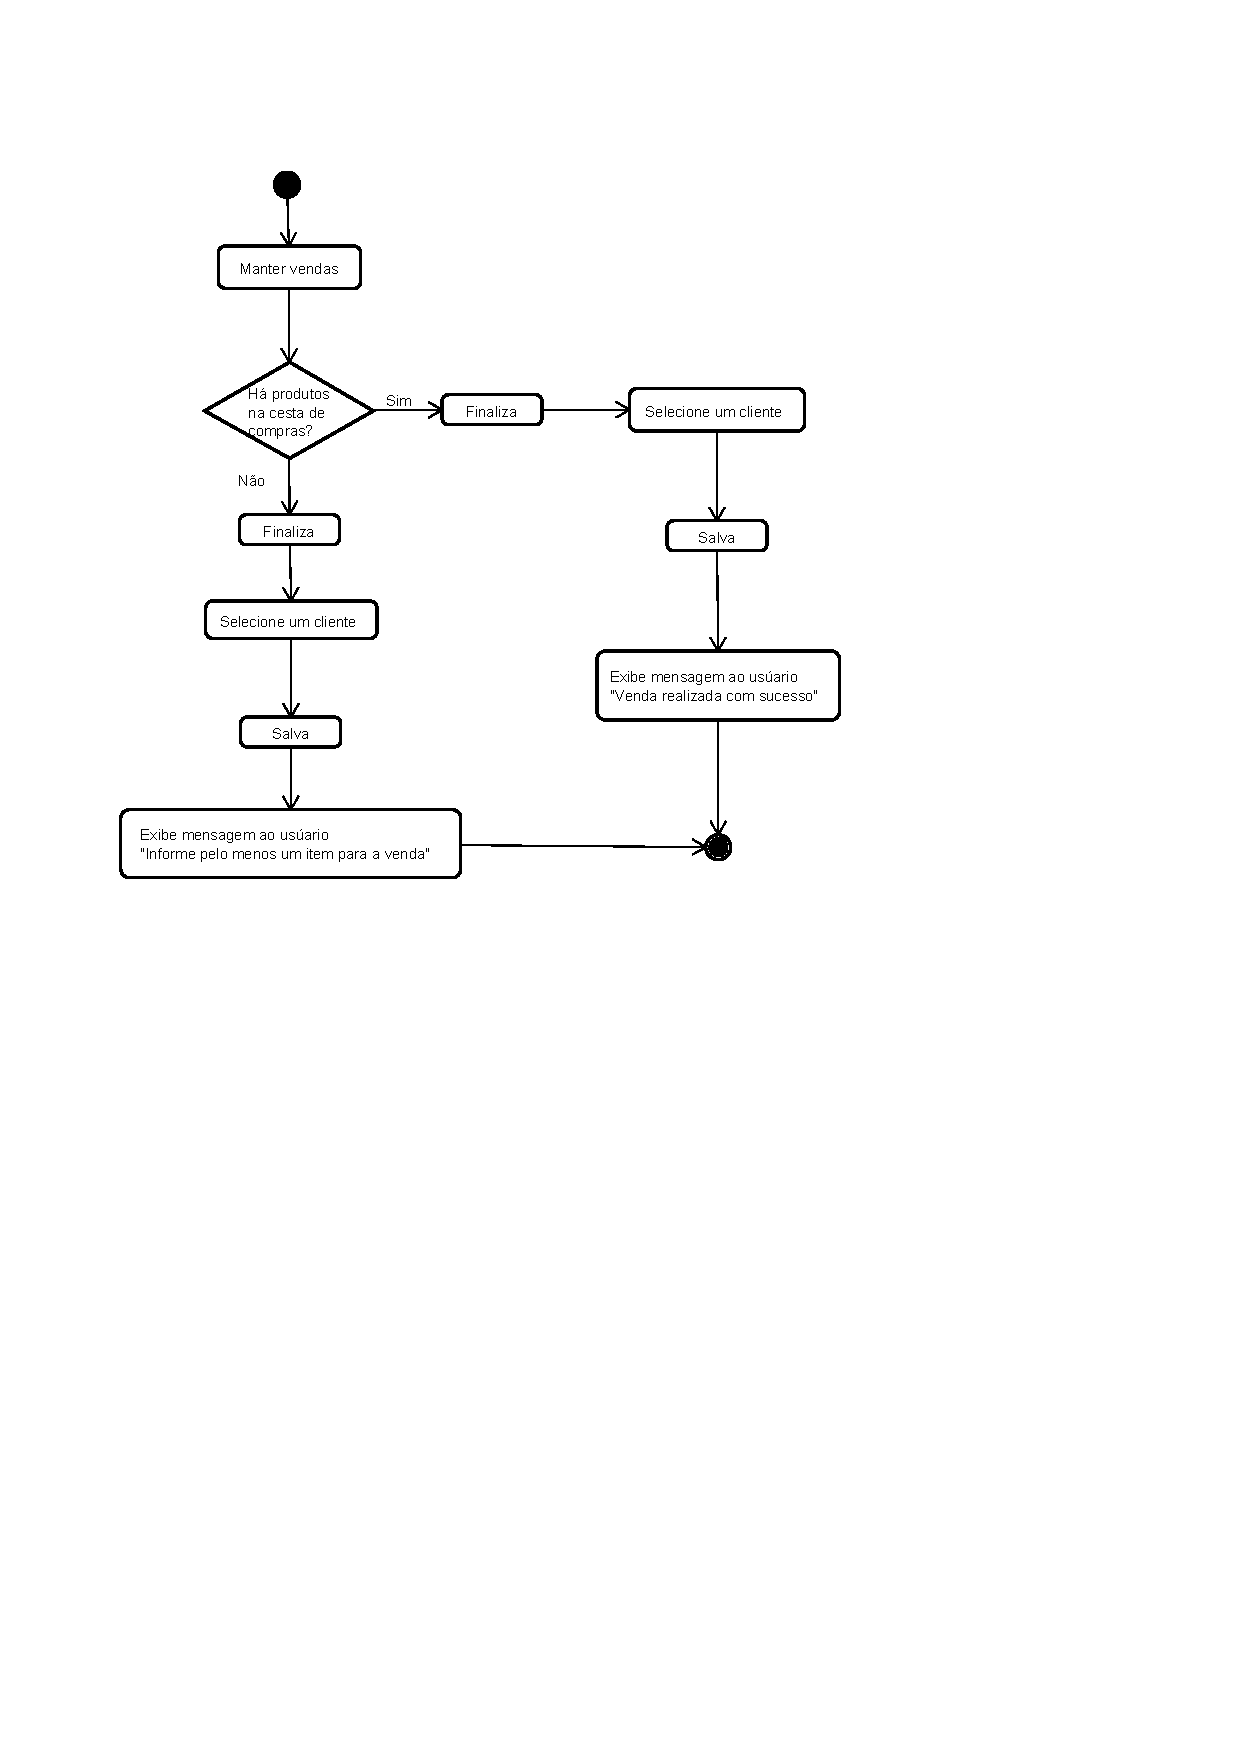
\includegraphics[scale=1.29]{venda.pdf}\caption{Manter venda}
\end{figure}

\newpage
\section{Diagrama de Entidades e Relacionamentos}
\begin{figure}[h]\centering
	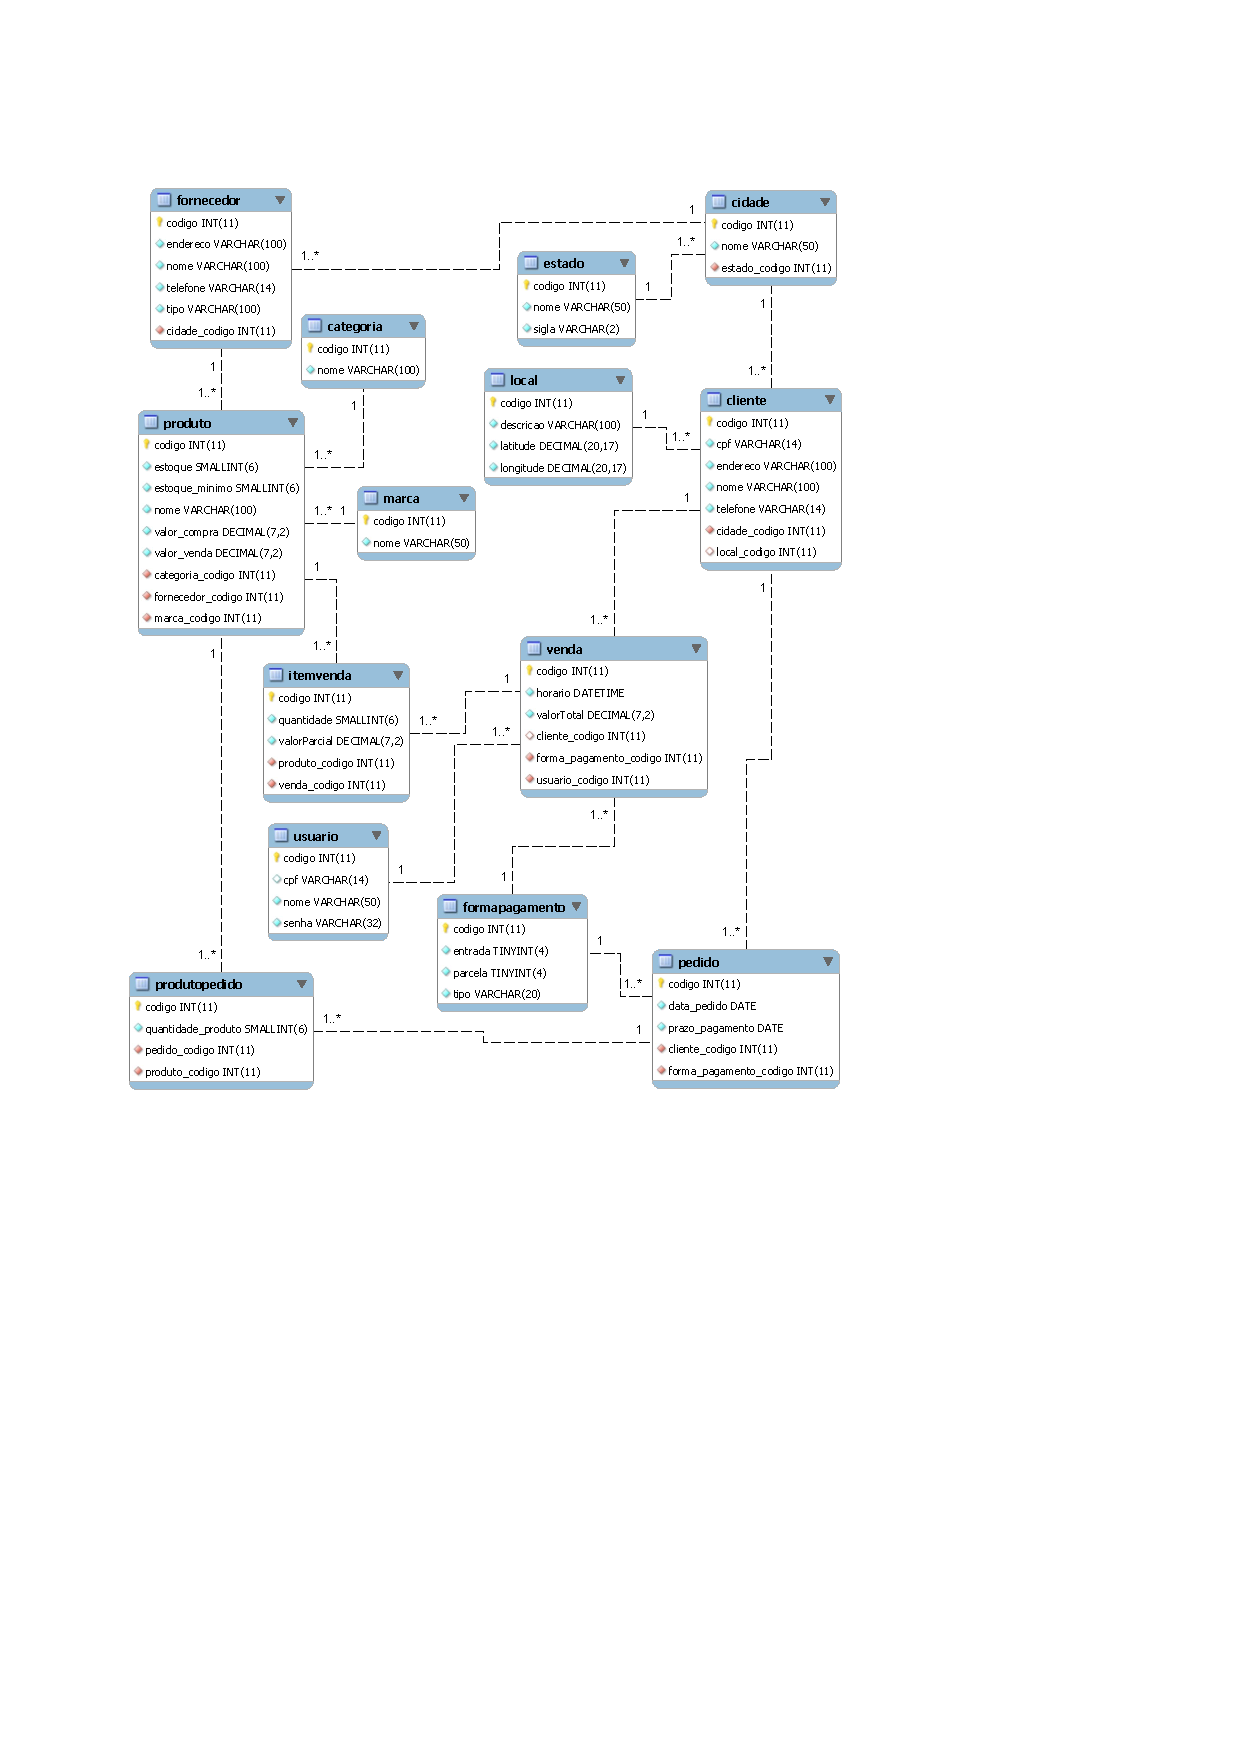
\includegraphics[scale=1.29]{der.pdf}\caption{DER – Diagrama de Entidades e Relacionamentos}
\end{figure}

%=================================
\chapter{Considerações Finais}
Diante do que foi exposto, fica evidente que o objetivo desse projeto para desenvolver um sistema de gestão de venda foi alcançado. O mesmo poderá proporcionar inúmeros benefícios ao usuário final, especificamente aos revendedores autônomos nas suas atividades, proporcionando um gerenciamento eficaz nos processos financeiros, armazenamento de informações e, possibilitando a monitoração dos serviços prestados.

Dentro do contexto atual da economia de mercado, na qual há maior movimentação de mercadorias e demanda de clientes, tornou- se necessário à utilização de um sistema informatizado. Com o método tradicional, não seria possível suprir de forma ágil, simples e segura o processo de venda. Assim como foi apontado no início do trabalho, grande parte das informações é registrada manualmente, as quais poderiam ser danificadas ou perdidas facilmente.

O projeto agregou inúmeros conhecimentos a equipe de desenvolvedores tanto na área da programação, engenharia de software e analise de sistemas.

Mesmo que o sistema desenvolvido atualmente possua numerosas e  interessantes funcionalidades para os revendedores, ainda são possíveis futuras expansões. Uma das futuras implementações poderia ser, por exemplo, a disponibilização para o usuário de mapas geográficos com apresentação de localizações de clientes e gráfico de estatísticas das vendas mensais.

Além disso, o sistema futuramente poderia vir apresentar uma integração com o sistema de login e de pagina comerciais do Facebook.

Considerando também o domínio no mercado de dispositivos moveis conectados a internet, seria interessante o desenvolvimento de uma versão para android, ios ou Windows phone. Isto permitiria ao revendedor a portabilidade do sistema e das informações contidas sobre as vendas.

%============================================================================
%\renewcommand{\bibname}{REFERÊNCIAS}
\begin{thebibliography}{99}
\vspace{-0.5cm}
ABEVD, Venda direta. Disponível em: $<$http://www.abevd.org.br/venda-direta$>$. Acesso em  23 mar. 2016.
\\[0,4cm]

AGENDOR. Disponível em: $<$http://www.agendor.com.br/blog/ate-onde-vendas-e-tecnologia-andam-juntas$>$ Acesso em  25 abr. 2016.
\\[0,4cm]

CIRIACO, F. Textos Técnicos com LaTeX: Disciplina de Trabalho de Conclusão de Curso. Disponivel em: $<$https://www.passeidireto.com/arquivo/3561661/apostila$>$. Acesso em: 01 mar. 2016.
\\[0,4cm]

DEITEL, Paul. J.; DEITEL, Harvey. M. {\em Java: como programar.} 8.ed. São Paulo: Pearson Prentice Hall, 2010.
\\[0,4cm]

DEVMEDIA. Padrão de Projeto Facade em Java. Higor Medeiros. Disponível em: $<$http://www.devmedia.com.br/padrao-de-projeto-facade-em-java/26476$>$ Acesso em  20 abr. 2016.
\\[0,4cm]

DOCPLAYER. Sistema de informacao destinado a gestao comercial de uma empresa do ramo alimenticio. Disponível em: $<$http://docplayer.com.br/2423163-Sistema-de-informacao-destinado-a-gestao-comercial-de-uma-empresa-do-ramo-alimenticio.html$>$ Acesso em  14 abr. 2016.
\\[0,4cm]

ELMASRI, Ramez; NAVATHE, Shamkant B. {\em Sistemas de banco de dados.} 6.ed. São Paulo: Pearson Addison Wesley, 2011.
\\[0,4cm]

MARIOPERSONA. Disponível em: $<$http://mariopersona.com.br/entrevista\_vendamais\_tecnologia.html$>$ Acesso em  30 abr. 2016.
\\[0,4cm]

PRIMEFACES. Disponível em: $<$http://www.primefaces.org/showcase/index.xhtml$>$ Acesso em  05 abr. 2016.
\\[0,4cm]

PORTAL EDUCAÇÃO. {O uso de tecnologia em vendas}. Disponivel em: $<$http://www.portaleducacao.com.br/administracao/artigos/36584/o-uso-de-tecnologia-em-vendas$>$. Acesso em: 15 abr. 2016.
\\[0,4cm]

PROGRAMAÇÃO WEB COM JAVA. Sérgio Roberto Delfino. Disponível em: $<$https://www.youtube.com/channel/UCJdtabTp9TXaHxdYrAa2j0A$>$. Acesso em  01 abr. 2016.
\\[0,4cm]
\end{thebibliography}
\end{document} 